\documentclass[a4paper,11pt]{article}
\usepackage[T1]{fontenc}
\usepackage[utf8]{inputenc}
\usepackage{lmodern}
\usepackage[margin=2.4cm]{geometry}
\usepackage{amsmath,amssymb}
\usepackage{graphicx}
\usepackage{booktabs}
\usepackage{tabularx}
\usepackage{longtable}
\usepackage{xcolor}
\usepackage{listings}
\usepackage{tikz}
\usetikzlibrary{arrows.meta,positioning,fit,calc}
\usepackage{siunitx}
\usepackage{caption}
\usepackage[hidelinks]{hyperref}

\graphicspath{{figures/}}
\sisetup{group-separator={,},group-minimum-digits=4}

\definecolor{codebg}{HTML}{F6F5F2}
\definecolor{codekw}{HTML}{2A78D6}
\definecolor{codecm}{HTML}{6E6D68}
\definecolor{codestr}{HTML}{B4501F}
\lstset{
  language=Python, basicstyle=\ttfamily\footnotesize, backgroundcolor=\color{codebg},
  keywordstyle=\color{codekw}\bfseries, commentstyle=\color{codecm}\itshape,
  stringstyle=\color{codestr}, frame=none, columns=fullflexible, keepspaces=true,
  breaklines=true, showstringspaces=false, xleftmargin=0.6em, framexleftmargin=0.6em,
  aboveskip=0.8em, belowskip=0.8em, upquote=true
}
\usepackage{xurl}
\DeclareUrlCommand\code{\urlstyle{tt}}
\newcommand{\Qfc}{Q_{fc}}
\newcommand{\Qext}{Q_{ext}}

\title{PhlyGreen Technical Manual: Thermal Management\\[4pt]
\large Theory, implementation and usage of the PEM fuel-cell system model}
\author{PhlyGreen development team\\Sapienza University of Rome}
\date{Code state: November 2026, branch \texttt{main}}

\begin{document}
\maketitle

\begin{abstract}
\noindent This manual documents the thermal-management system (TMS) of the fuel-cell
configurations of PhlyGreen. The TMS rejects the heat that the fuel-cell stack produces. We
describe the two model classes. Class~I converts the peak heat into a mass with a specific
power. Class~II sizes a coolant loop with geometric heat exchangers, a pump and a ram-air
duct, chooses its design point over the mission, and feeds the pump power and the duct drag
back into the aircraft sizing loop. For each part we give the theory, the implementation and
the inputs. Every number in the manual comes from running the code on the reference
configurations of \code{trunk/examples/common.py}. The scripts that produce the numbers and
the figures are in \code{manuals/tms/scripts/}.
\end{abstract}

\tableofcontents
\newpage

%% ======================================================================================
\section{Scope and overview}\label{sec:scope}
%% ======================================================================================

A proton-exchange-membrane (PEM) fuel cell converts roughly half of the hydrogen energy
into electricity. The rest becomes heat at the stack operating temperature $T_{op}$, which
is \SI{353.15}{K} (\SI{80}{\celsius}) for the stacks of the PhlyGreen database used in this
manual. The thermal-management system (TMS) must reject this heat. Because the temperature
difference to the ambient air is small, the TMS is heavy, it needs a coolant pump, and its
ram-air duct can add drag. Therefore the TMS is part of the aircraft sizing problem and not
a separate post-processing step.

This manual covers heat \emph{rejection}. It describes how PhlyGreen turns the stack heat
into a TMS mass, a pump power and a duct drag, and how these quantities feed back into the
take-off-weight closure. The heat \emph{generation} in the stack (polarization curve, heat
basis, product-water phase) belongs to the companion manual \emph{PhlyGreen Technical
Manual: Fuel Cell}. Section~\ref{sec:heat-source} only summarizes it. The battery cooling
mass of the hybrid closures belongs to \emph{PhlyGreen Technical Manual: Battery}; we
mention it in Section~\ref{sec:battery-hex}.

PhlyGreen offers two TMS model classes for the two fuel-cell configurations,
\code{'Hydrogen'} and \code{'FuelCellBattery'}:
\begin{itemize}
\item \textbf{Class I} (default). The TMS mass is the peak stack heat divided by a specific
  power. There is no drag and no pump power.
\item \textbf{Class II}. A geometric model of a coolant loop. The coolant first warms the
  liquid hydrogen fuel and then rejects the rest of the heat to ram air. Each heat exchanger
  is sized from its geometry. The model returns the exchanger and pump masses, the pump
  power and the ram-air duct drag. It chooses its design point over the mission.
\end{itemize}

\paragraph{Where the code lives.} Table~\ref{tab:files} lists the files. The subsystem is
attached to the aircraft as \code{aircraft.tms} by \code{PhlyGreen/factory.py:build_aircraft}.
It reads its inputs in \code{TMS.py:ThermalManagementSystem.SetInput} from
\code{aircraft.TMSInput}, which is the dictionary form of \code{config/sections.py:TMSConfig}.

\begin{table}[htbp]
\centering\small
\caption{Source files of the thermal-management system (paths relative to
\texttt{trunk/PhlyGreen/}).}\label{tab:files}
\begin{tabularx}{\textwidth}{@{}lX@{}}
\toprule
File & Content \\
\midrule
\code{Systems/Thermal/TMS.py} & \code{ThermalManagementSystem} (Class I and II), \code{FCThermalManagementResult}, \code{ExchangerUnit} \\
\code{Systems/Thermal/hex.py} & fluid streams, $\varepsilon$-NTU, the three exchanger families, family selection, rating \\
\code{Systems/Thermal/ram_air.py} & \code{ram_air_drag}: net drag of the ram-air duct \\
\code{Systems/Thermal/plotting.py} & \code{draw_hex}, \code{plot_tms_rating} \\
\code{Systems/Thermal/network.py} & heat-source/sink scaffold for studies (not used by the sizing) \\
\code{Mission/Mission.py} & \code{thermal_profile}, \code{_takeoff_fc_heat}, \code{_begin_thermal_phase}, \code{_end_thermal_phase}, \code{_track_fc_heat} \\
\code{Weight/Weight.py} & \code{_fuel_cell_and_tms_closure}, \code{_fuel_cell_tms_mass}, \code{_warn_tms_shortfall}, \code{Hydrogen}, \code{FuelCellBattery} \\
\code{Systems/FuelCell/FuelCell.py} & \code{Q_thermal}, \code{P_aux_tms} \\
\code{Systems/Aerodynamics/Aerodynamics.py} & \code{extra_Cd} added in \code{Cd} \\
\code{config/sections.py} & \code{TMSConfig}; \code{EnergyConfig.hex_specific_power_h2}, \code{hex_specific_power_battery} \\
\code{results.py} & \code{tms_class}, \code{tms_mass}, \code{hex_mass}, \code{tms_pump_power}, \code{tms_ram_drag}, \code{tms_design_point}, \code{fuelcell_rating}, \code{empty_weight} \\
\bottomrule
\end{tabularx}
\end{table}

\paragraph{Reference designs.} All numbers in this manual come from the scripts in
\code{manuals/tms/scripts/}. They use the configurations of
\code{trunk/examples/common.py}:
\begin{itemize}
\item \textbf{H2}: \code{hydrogen_config(tms_class=...)}, an ATR-like fuel-cell aircraft with
  \SI{4560}{kg} payload, a \SI{750}{nmi} mission and a \SI{220}{nmi} diversion, the
  \code{PEMFC_GoodPerformance} stack at a design cell voltage of \SI{0.5}{V}, and a
  gravimetric-index hydrogen tank;
\item \textbf{FCB}: \code{fuelcell_battery_config(tms_class=...)}, the same aircraft with a Class-I
  battery that supplies 15\,\% of the cruise power (cruise $\phi = 0.15$);
\item \textbf{FCB-800}: \code{examples/30_off_design_mission.py:fc_battery_design()},
  the FCB aircraft with $\phi = 0$ in flight, $\phi = 0.15$ at take-off and an
  \SI{800}{m} take-off field. The taxi legs take the take-off $\phi$, the default of
  \code{MissionConfig.taxi_phi}. It is used only for the take-off over-temperature and the
  degradation study.
\end{itemize}
Unless stated otherwise the TMS inputs are the defaults of Table~\ref{tab:inputs}.

%% ======================================================================================
\section{The heat source}\label{sec:heat-source}
%% ======================================================================================

The TMS rejects the heat that the fuel-cell model reports. This section summarizes how
that heat is computed and where it is sampled. The details are in the fuel-cell manual.

\subsection{Stack heat on the coolant basis}
At every operating point \code{FuelCell.ComputePRatio} solves the stack current for the
required electrical power and stores the stack heat as \code{fc.Q_thermal}
(\code{FuelCell.py}, lines 728--731):
\begin{equation}
  \Qfc = I\,N_{cells}\left[\frac{\Delta H_{HHV} - x_v\,(\Delta H_{HHV} - \Delta H_{LHV})}{2F} - V_{cell}\right],
  \label{eq:qfc}
\end{equation}
where $I$ is the cell current, $N_{cells}$ the number of cells, $F$ the Faraday constant,
$V_{cell}$ the cell voltage, $\Delta H_{HHV}$ and $\Delta H_{LHV} = \SI{241.8}{kJ/mol}$ the
reaction enthalpies with liquid and vapour product water, and $x_v$ the fraction of the
product water that leaves the stack as vapour. Vapour carries its latent heat away with the
cathode exhaust, so that heat does not reach the coolant. By default
\code{FuelCell.vapour_fraction_at} evaluates $x_v$ at every operating point from the
saturation of the cathode exhaust (\code{product_water_vapour_fraction}), given the
relative humidity of the cathode inlet. That humidity is the larger of the humidifier
setting \code{EnergyConfig.fc_cathode_inlet_rh} and the humidity that the compressor
carries in from the ambient air, \code{EnergyConfig.fc_ambient_relative_humidity}
(\code{FuelCell.cathode_inlet_rh}). Both default to zero. For the dry stack of the
reference designs ($T_{op} = \SI{80}{\celsius}$, \SI{1.5}{bar}, air stoichiometry
$\lambda = 2$) the code returns $x_v = 1$. The coolant then sees the
lower-heating-value basis: the bracket in~\eqref{eq:qfc} is the thermo-neutral voltage on
the LHV basis minus the cell voltage. The input
\code{EnergyConfig.fc_product_water_vapour_fraction} fixes $x_v$ instead. The hydrogen
consumption does not depend on $x_v$. The fuel-cell ambient state follows the mission
temperature offset (DISA), as the TMS ambient does. 

Humidity changes the heat. With a humidifier that saturates the cathode inlet
(\code{fc_cathode_inlet_rh} = 1) the exhaust cannot take up the product water, so $x_v = 0$
and the coolant sees the HHV basis. On \code{hydrogen_config(tms_class='I')} this raises the
take-off heat from \SI{4018}{kW} to \SI{5622}{kW} (+40\,\%), the Class-I TMS mass from
\SI{940}{kg} to \SI{1289}{kg} (+37\,\%) and the take-off mass from \SI{21634}{kg} to
\SI{22662}{kg} (+4.8\,\%). The weather humidity has a negligible effect: an ambient relative
humidity of 0.6 or 1.0 changes the Class-I TMS mass by less than \SI{0.3}{kg}, because the
cold ambient air carries little water compared with the saturation capacity at
\SI{80}{\celsius}. The reference designs of this manual use dry air and no humidifier.

When the TMS pump load is active (Class~II, Section~\ref{sec:coupling}), the electrical
power of the stack includes the pump power \code{fc.P_aux_tms}. The heat in~\eqref{eq:qfc}
therefore includes the heat produced to drive the pump.

\subsection{The mission thermal profile}\label{sec:profile}
The TMS is sized and rated on a list of heat-load points, \code{mission.thermal_profile}.
Each point is a dictionary \texttt{\{name, Q\_fc [W], altitude [m], V\_inf [m/s TAS], mdot\_h2 [kg/s]\}}. The list is built by \code{Mission.HydrogenConfiguration} and
\code{Mission.FuelCellBatteryConfiguration} in two steps:
\begin{enumerate}
\item \code{Mission._takeoff_fc_heat} evaluates the fuel cell at the worst-case
  off-mission propulsive power, the larger of the take-off and one-engine-inoperative
  (OEI) climb powers (\code{Mission._worst_case_propulsive_power}), at the altitude and
  speed of the take-off constraint. For a fuel-cell + battery aircraft only the fuel-cell
  share $(1-\phi_{TO})$ of that power is used. This point is not flown by the profile. It
  becomes the first entry, named \code{'Takeoff'}, with the flag \texttt{takeoff = True}. If
  the battery covers the whole take-off power the list starts empty.
\item During the time integration, \code{_begin_thermal_phase} and
  \code{_end_thermal_phase} bracket each flight segment. After the integrator has solved a
  segment, \code{_track_fc_heat_on_solution} re-evaluates the fuel cell at the accepted
  solver points of that segment, and \code{_track_fc_heat} records the largest $\Qfc$
  in the segment together with its altitude, speed and hydrogen flow. Each
  segment with a positive peak adds one entry, named \code{'<phase>/<segment>'} (for
  example \code{'Mission/Climb1'} or \code{'Diversion/Cruise'}).
\end{enumerate}
The scalars \code{mission.TO_FC_Thermal_Pwr} and \code{mission.Max_FC_Thermal_Pwr} hold the
take-off heat and the in-flight peak.

The peaks are therefore sampled at the accepted solver points only, not at the trial
evaluations of the integrator. The taxi and take-off-run ground segments (\code{Mission._ground_segments}) are not part of the
thermal profile.

\subsection{Battery cooling}\label{sec:battery-hex}
The TMS of this manual serves the fuel cell only. A Class-II battery has its own cooling
mass term in \code{Weight.Hybrid} and \code{Weight.FuelCellBattery}: the peak in-flight
battery waste heat \code{mission.Max_Bat_Thermal_Pwr} divided by
\code{EnergyConfig.hex_specific_power_battery} (default \SI{1500}{W/kg}). In the
fuel-cell + battery closure this term is added to \code{weight.WHeat_Exchanger} after the
fuel-cell TMS mass, so \code{results().tms_mass} and \code{results().hex_mass}, which both
report \code{weight.WHeat_Exchanger}, include it when the battery is Class~II.
The battery manual describes the battery heat.

%% ======================================================================================
\section{Class I: specific-power model}\label{sec:class1}
%% ======================================================================================

Class~I converts the peak heat into a mass with one technology constant. In
\code{Weight._fuel_cell_tms_mass} and \code{TMS.ClassI_Mass},
\begin{equation}
  W_{TMS}^{I} = \frac{\max\left(Q_{fc,\,mission\ peak},\; Q_{fc,\,take\text{-}off}\right)}{s_{HEX}},
  \label{eq:class1}
\end{equation}
with $s_{HEX}$ = \code{EnergyConfig.hex_specific_power_h2} (legacy key
\texttt{'HEX Specific Power H2'}, default \SI{5000}{W/kg}). The take-off point is included
because the fuel cell is sized there and often rejects the most heat there. The default is
a model assumption. Marconi~\cite{marconi2026} reports that a specific heat rejection of
\SI{5}{kW/kg} corresponds to a 2050 technology horizon in the ATI FlyZero thermal-management
roadmap~\cite{flyzero}, and \SI{2.5}{kW/kg} to a 2030--2035 horizon. The thesis writes the
same model as $Q_{max}/(k_{TMS}\,\Delta T_{sizing})$ with a specific conductance $k_{TMS}$;
PhlyGreen uses the specific power directly.

Class~I has no geometry. It does not depend on altitude or speed, so it cannot see that a
slow, hot point is harder to cool than a fast, cold one. It adds no drag and no pump power.

%% ======================================================================================
\section{Class II: theory and implementation}\label{sec:class2}
%% ======================================================================================

Class~II sizes the hardware of a single coolant loop at one design point, then rates that
hardware at the other mission points. This section describes the sizing at one point. The
choice of the design point is the subject of Section~\ref{sec:design-point}.

\subsection{Loop architecture}\label{sec:architecture}
Figure~\ref{fig:loop} shows the architecture (module docstring of \code{TMS.py}). The
coolant, by default the CoolProp incompressible fluid \texttt{'INCOMP::MEG-30\%'} (a
monoethylene-glycol/water mixture with 30\,\% glycol), leaves the stack at $T_{op}$. It
crosses two exchanger roles in series:
\begin{enumerate}
\item \textbf{HEX~1}, role \code{'coolant_to_h2'}: the coolant warms the hydrogen fuel
  from saturated liquid at the supply pressure to $T_{op} - \Delta T_{H_2}$;
\item \textbf{HEX~2}, role \code{'coolant_to_ram_air'}: the coolant rejects the remaining
  heat to ram air captured by an intake.
\end{enumerate}
A pump closes the loop. The coolant returns to the stack $\Delta T_{loop}$ colder than it
left. Each role may consist of several identical units in parallel
(Section~\ref{sec:parallel}).

\begin{figure}[htbp]
\centering
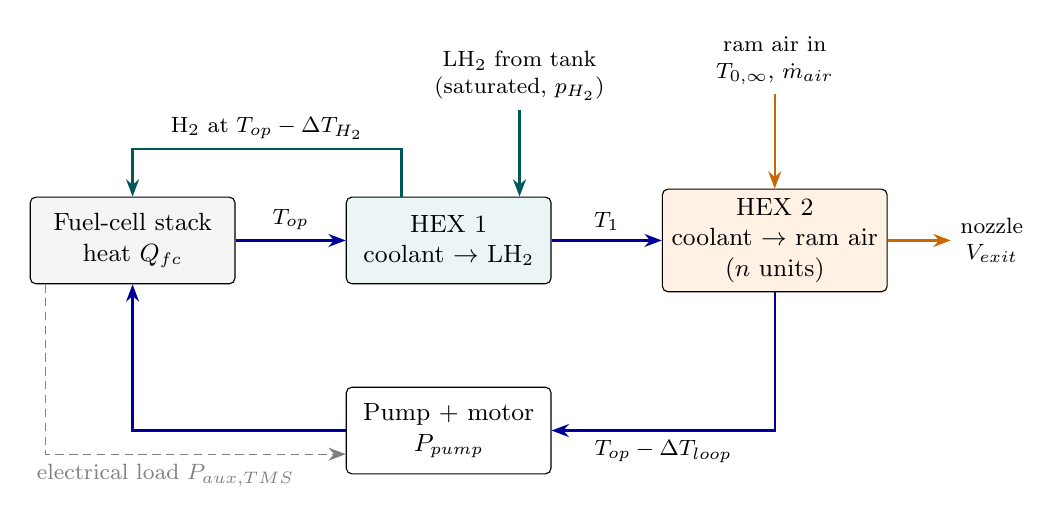
\begin{tikzpicture}[
  >={Stealth[length=2.2mm]}, node distance=9mm and 14mm,
  box/.style={draw, rounded corners=2pt, minimum width=26mm, minimum height=11mm,
              align=center, font=\small, fill=#1},
  box/.default=white,
  lbl/.style={font=\footnotesize, align=center},
  cool/.style={->, thick, draw=blue!60!black},
  hyd/.style={->, thick, draw=teal!70!black},
  air/.style={->, thick, draw=orange!80!black}]
  \node[box=gray!8] (stack) {Fuel-cell stack\\ heat $\Qfc$};
  \node[box=teal!8, right=of stack] (hx1) {HEX 1\\ coolant $\to$ LH$_2$};
  \node[box=orange!10, right=of hx1] (hx2) {HEX 2\\ coolant $\to$ ram air\\ ($n$ units)};
  \node[box, below=13mm of hx1] (pump) {Pump + motor\\ $P_{pump}$};
  % coolant loop
  \draw[cool] (stack) -- node[lbl, above] {$T_{op}$} (hx1);
  \draw[cool] (hx1) -- node[lbl, above] {$T_1$} (hx2);
  \draw[cool] (hx2.south) |- node[lbl, pos=0.75, below] {$T_{op}-\Delta T_{loop}$} (pump.east);
  \draw[cool] (pump.west) -| (stack.south);
  % hydrogen
  \node[lbl, above=11mm of hx1, xshift=9mm] (lh2) {LH$_2$ from tank\\ (saturated, $p_{H_2}$)};
  \draw[hyd] (lh2.south) -- ([xshift=9mm]hx1.north);
  \draw[hyd] ([xshift=-6mm]hx1.north) -- ++(0,6mm) -| (stack.north);
  \node[lbl, anchor=south] at ($(stack.north)!0.5!([xshift=-6mm]hx1.north)+(0,6mm)$) {H$_2$ at $T_{op}-\Delta T_{H_2}$};
  % ram air
  \node[lbl, above=12mm of hx2] (ramin) {ram air in\\ $T_{0,\infty}$, $\dot m_{air}$};
  \draw[air] (ramin) -- (hx2.north);
  \node[lbl, right=8mm of hx2] (ramout) {nozzle\\ $V_{exit}$};
  \draw[air] (hx2.east) -- (ramout);
  % electrical
  \draw[->, densely dashed, gray] (stack.south west) ++(2mm,0) |- node[lbl, pos=0.7, below]
     {electrical load $P_{aux,TMS}$} ([yshift=-3mm]pump.west);
\end{tikzpicture}
\caption{Class-II loop (FC\_SPEC architecture). Coolant in blue, hydrogen in green,
ram air in orange. The pump is an electrical load on the fuel cell. The hydrogen leaves
HEX~1 at $T_{op}-\Delta T_{H_2}$ and is warmed to $T_{op}$ inside the stack.}
\label{fig:loop}
\end{figure}

\subsection{Heat balance at one point}\label{sec:balance}
\code{TMS._conditions} computes the heat split at a mission point. The ambient static
temperature $T_\infty$, pressure $p_\infty$ and density $\rho_\infty$ come from the ISA
model plus the mission temperature offset (\code{TMS._ambient}). The coolant temperature is
$T_{op}$, increased by the take-off over-temperature $\Delta T_{TO}$ at the take-off point
only (Section~\ref{sec:overtemp}).

\paragraph{Hydrogen stream.} The hydrogen enters HEX~1 as saturated liquid (\SI{21.9}{K} at the
default pressure, from CoolProp) at the supply
pressure $p_{H_2}$ (default \SI{1.6}{bar}) and leaves at $T_{H_2,out} = T_{op} -
\Delta T_{H_2}$ (default approach $\Delta T_{H_2} = \SI{30}{K}$). Para-hydrogen
enthalpies from CoolProp give the duty of HEX~1,
\begin{equation}
  q_{1}^{*} = \dot m_{H_2}\,\big[h(T_{H_2,out}, p_{H_2}) - h_{sat,liq}(p_{H_2})\big],
  \label{eq:q1}
\end{equation}
which includes the latent heat of vaporization. For the $\varepsilon$-NTU method the
hydrogen is given an \emph{effective} specific heat
$c_{p,eff} = [h(T_{H_2,out}) - h_{sat,liq}]/(T_{H_2,out} - T_{sat})$, so that
$\dot m\,c_{p,eff}\,\Delta T$ is the exact enthalpy rise. Its transport properties are taken
at the mean temperature $(T_{sat} + T_{H_2,out})/2$.

\paragraph{Reactant heat.} The hydrogen is then warmed from $T_{H_2,out}$ to $T_{op}$, and
the cathode air from the compressor delivery temperature to $T_{op}$, inside the stack. This
heat is absorbed by the reactants and does not reach the coolant:
\begin{equation}
  q_{react} = \dot m_{H_2}\,\big[h(T_{op}) - h(T_{H_2,out})\big]
            + \dot m_{air}\,c_{p,air}\,(T_{op} - T_{comp}).
  \label{eq:qreact}
\end{equation}
The cathode-air flow follows from the hydrogen flow and the stoichiometry $\lambda$, and
the compressor delivery temperature from an adiabatic compression of ambient air:
\begin{equation}
  \dot m_{air} = \frac{\dot m_{H_2}}{M_{H_2}}\,\frac{0.5}{0.21}\,M_{air}\,\lambda,
  \qquad
  T_{comp} = T_\infty\left[1 + \frac{\Pi^{0.4/1.4} - 1}{\eta_{comp}}\right],
\end{equation}
with $\Pi = \max(p_{cathode}/p_\infty, 1)$ and the compressor efficiency $\eta_{comp}$ of the
fuel-cell model. If $T_{comp} > T_{op}$ the air term is negative, so the reactants add heat.
The coolant must reject
\begin{equation}
  \Qext = \max(\Qfc - q_{react},\,0),
\end{equation}
and the duty of HEX~1 is $q_1 = \min(q_1^{*}, \Qext)$.

\paragraph{Coolant flow.} The coolant flow is fixed at the design point by the loop
temperature drop $\Delta T_{loop}$ (default \SI{10}{K}),
\begin{equation}
  \dot m_c = \frac{\Qext}{c_{p,c}\,\Delta T_{loop}},
\end{equation}
with the coolant properties evaluated at $T_{op}$ and \SI{2}{bar} (\code{TMS._coolant}).
The coolant leaves HEX~1 at $T_1 = T_{op} - q_1/(\dot m_c c_{p,c})$.

\paragraph{Ram-air stream.} HEX~2 rejects $q_2 = \Qext - q_1$. The ram air enters the core
at the free-stream total temperature $T_{0,\infty} = T_\infty + V_\infty^2/(2c_p)$ with
$c_p = \SI{1005}{J/(kg\,K)}$. Its design temperature rise is
\begin{equation}
  \Delta T_{air} = \min\big(\Delta T_{air,design},\; \varepsilon_{max}\,(T_1 - T_{0,\infty})\big),
  \label{eq:dtair}
\end{equation}
with $\Delta T_{air,design}$ = \code{ram_air_delta_t} (default \SI{50}{K}) and
$\varepsilon_{max}$ = \code{ram_air_max_effectiveness} (default 0.8). The cap keeps the
required effectiveness below $\varepsilon_{max}$ when the driving temperature difference is
small. The ram-air flow follows as $\dot m_{air} = q_2/(c_{p,air}\,\Delta T_{air})$, with
the air properties at $T_{0,\infty} + \Delta T_{air,design}/2$. The intake capture area
is $A_{cap} = \dot m_{air}/(\rho_\infty V_\infty)$.

\subsection{The $\varepsilon$-NTU method}\label{sec:entu}
Each exchanger is sized and rated with the effectiveness--number of transfer units method
(\code{hex.py}, section~2). With the heat-capacity rates $C = \dot m c_p$,
$C_{min}$ and $C_{max}$, the capacity ratio $C_r = C_{min}/C_{max}$ and the overall
conductance $UA$, the number of transfer units is $NTU = UA/C_{min}$. The effectiveness
\begin{equation}
  \varepsilon = \frac{q}{C_{min}\,(T_{h,in} - T_{c,in})}
\end{equation}
is a closed-form function of $NTU$, $C_r$ and the flow arrangement
(\code{hex.py:effectiveness}, Incropera and DeWitt, Table~11.3~\cite{incropera}):
\begin{align}
  \text{counterflow:}&\quad \varepsilon = \frac{1 - e^{-NTU(1-C_r)}}{1 - C_r\,e^{-NTU(1-C_r)}}
    \quad(\varepsilon = NTU/(1+NTU) \text{ if } C_r = 1),\\
  \text{cross-flow, } C_{max}\text{ mixed:}&\quad \varepsilon = \frac{1}{C_r}\left[1 - e^{-C_r(1 - e^{-NTU})}\right],\\
  \text{cross-flow, } C_{min}\text{ mixed:}&\quad \varepsilon = 1 - \exp\!\left[-\frac{1}{C_r}\left(1 - e^{-C_r NTU}\right)\right],
\end{align}
plus the parallel-flow and both-unmixed cross-flow relations, which the families do not
use. For $C_r \to 0$ every arrangement gives $\varepsilon = 1 - e^{-NTU}$. For the tube
banks the gas crossing the bank is the mixed stream. \code{crossflow_one_mixed} picks the
$C_{min}$-mixed or $C_{max}$-mixed relation from the heat-capacity rates.

The method serves both problems:
\begin{itemize}
\item \textbf{Sizing.} The duty fixes $\varepsilon$. \code{ntu_required} inverts
  $\varepsilon(NTU)$ by bisection on $[0, 50]$ and raises an error when $\varepsilon$ is not
  reachable. The required reference area is $A = NTU\,C_{min}/U$
  (\code{HeatExchangerSizer._area_for}).
\item \textbf{Rating.} For a built geometry, $U$ follows from the flows,
  $NTU = UA/C_{min}$, and \code{thermal_solve} returns
  $q = \varepsilon\,C_{min}\,(T_{h,in} - T_{c,in})$.
\end{itemize}
The thesis~\cite{marconi2026} reviews the log-mean-temperature-difference method and adopts
$\varepsilon$-NTU as the only routine, because rating then needs no iteration on the outlet
temperatures. The code follows the same choice.

\subsection{Exchanger families}\label{sec:families}
Three families are implemented as subclasses of \code{HeatExchangerSizer}. Each family
defines a grid of candidate geometries, a \emph{layout} rule that turns a geometry and a
reference area into a built core, a \code{compute_U} method that returns $U$, the
velocities and the pressure drops of a built core at given flows, and a mass and volume
rule. Table~\ref{tab:families} summarizes them. In all families the coolant is the hot
stream inside the tubes or channels, and the hydrogen or the ram air is the cold stream.

\begin{table}[htbp]
\centering\small
\caption{Exchanger families of \texttt{hex.py}. ``Gas'' is the cold stream (ram air or
hydrogen).}\label{tab:families}
\begin{tabularx}{\textwidth}{@{}>{\raggedright\arraybackslash}p{2.6cm}>{\raggedright\arraybackslash}X>{\raggedright\arraybackslash}X>{\raggedright\arraybackslash}p{2.0cm}@{}}
\toprule
Family & Liquid side & Gas side & Arrangement \\
\midrule
\code{plain_tube_bank} (staggered, square pitch, steel tubes) &
  Gnielinski~\cite{gnielinski} with Petukhov $f$; laminar $Nu = 3.66$ &
  Zukauskas~\cite{zukauskas} $Nu = C_2\,C\,Re^m Pr^{0.36}$ with row correction $C_2$~\cite{incropera}; Jakob pressure drop as
  reported by Holman~\cite{holman} & cross-flow, gas mixed \\
\code{finned_tube_bank} (steel tubes, annular Al fins) &
  as above &
  Briggs \& Young~\cite{briggs} $Nu = 0.134\,Re^{0.681}Pr^{1/3}$ $\times(s/l)^{0.2}(s/t)^{0.1134}$; Schmidt fin
  efficiency; $f = 1.5\,Re^{-0.2}$ & cross-flow, gas mixed \\
\code{plate_fin} (brazed Al, offset-strip fins) &
  plain channel, Gnielinski; laminar $Nu = 7.54$ &
  Manglik \& Bergles~\cite{manglik} $j$ and $f$ factors & counterflow \\
\bottomrule
\end{tabularx}
\end{table}

\paragraph{Design velocities and layout.} The convective coefficient depends on the
velocity, the velocity on the flow area, and the flow area on the geometry. The code breaks
this circle with typical design velocities: \SI{1.75}{m/s} for liquids and \SI{15}{m/s}
for gases (\code{DESIGN_VELOCITY_LIQUID}, \code{DESIGN_VELOCITY_GAS}). A stream counts as
liquid when its density exceeds \SI{500}{kg/m^3} (\code{FluidStream.is_liquid}). Hence the
hydrogen stream, with properties at its mean temperature, uses the gas velocity. The
design velocities fix the flow areas. The required area then fixes the depth:
\begin{itemize}
\item \emph{Tube banks} (\code{_TubeBankSizer.layout}). The total tube length is
  $L_{tot} = A/a_o$, with $a_o$ the outer area per metre of tube. The face, $n_{row}\,L$
  tubes times length, is set so that the gas reaches its design velocity in the minimum
  flow area $n_{row}\,L\,(S_T - w_{block})$, with $S_T$ the transverse pitch and $w_{block}$
  the blocked width. The face is square ($n_{row} S_T \approx L$). The number of rows is
  $\lceil L_{tot}/(n_{row} L)\rceil$. On the liquid side, the number of parallel circuits
  gives the liquid design velocity, and the remaining tubes are in series. The wall is
  \SI{1}{mm} of stainless steel ($\rho = \SI{7800}{kg/m^3}$, $k = \SI{16}{W/(m\,K)}$). The
  candidate grid scans seven outer diameters from 6 to \SI{25}{mm}. For the plain bank the
  pitch ratio $S_T/d_o$ is 1.25, 1.5 or 2.0. For the finned bank the fin height is 6, 10 or
  \SI{14}{mm}, the fin density 450, 550 or 650 fins/m (fin thickness \SI{0.3}{mm}) and the
  pitch 1.05 or 1.20 times the fin diameter, so adjacent fins never overlap.
\item \emph{Plate-fin} (\code{PlateFinSizer.layout}). The number of layers follows from the
  larger of the gas and liquid layer counts at their design velocities, for a candidate
  core width. The liquid channel gap follows from the liquid flow. A gap below
  \SI{1}{mm} (\code{MIN_GAP_H}) is rejected as not producible. The flow length is
  $L = A/(\beta\,n_{layers}\,h\,w)$, with the gas-side area density
  $\beta = 2(s+h)/(sh)$, fin pitch $s$, fin height $h$ and width $w$. The grid scans three
  fin pitches, two fin heights, two strip lengths and four widths (0.1 to \SI{0.5}{m}).
\end{itemize}

\paragraph{Overall coefficient.} $U$ is referred to the gas-side reference area $A$
(\code{HEX_Design.A}); the liquid-side and wall resistances are scaled by the area ratio.
For the finned bank,
\begin{equation}
  \frac{1}{U} = \frac{A_o}{A_i\,h_{in}} + A_o\,R'_{wall} + \frac{1}{\eta_o\,h_{out}},
  \qquad \eta_o = 1 - \frac{A_{fin}}{A_o}(1 - \eta_f),
\end{equation}
with the inner and outer areas per metre $A_i$ and $A_o$, the wall resistance per metre
$R'_{wall} = \ln(d_o/d_i)/(2\pi k_{wall})$, and the fin efficiency $\eta_f =
\tanh(mr_1\phi)/(mr_1\phi)$ of Schmidt's equivalent-radius approximation. The plain bank is
the special case without fins. For the plate-fin core,
$1/U = (A_c/A_h)/h_h + (A_c/A_h)\,t_p/k + 1/(\eta_o h_c)$ with $A_c/A_h = (s+h)/s$. There
is no fouling resistance. This geometry-to-$h$-to-$UA$ chain follows the compact-surface
approach of Kays and London~\cite{kays}, as summarized by Marconi~\cite{marconi2026}.

\paragraph{Pressure drops.} The liquid side uses Darcy friction over the tube length times
the number of passes (tube banks) or over the flow length (plate-fin). The gas side uses
the Jakob correlation $\Delta p = 4f'N\rho V_{max}^2/2$ (plain bank), $N f \rho V_{max}^2/2$
with $f = 1.5\,Re^{-0.2}$ (finned bank), and $4f(L/D_h)\rho v^2/2$ with the Manglik and
Bergles $f$ (plate-fin). The code states that the finned-bank friction factor has no
literature source and recommends a validated correlation, such as Robinson and Briggs.

\paragraph{Mass and volume.} The mass is the material volume times the density: the
tubes (steel) and the fins (aluminium, $\rho = \SI{2700}{kg/m^3}$) of the tube banks, and
the fins and parting sheets (aluminium, \SI{0.5}{mm} plates, \SI{0.2}{mm} fins) of the
plate-fin core. The volume is the bounding box of the core. Headers, manifolds, piping,
ducts, coolant inventory and mounting structure are not included, so the mass is a
core-only figure.

\subsection{Self-consistent sizing and feasibility}\label{sec:selfconsistent}
\code{HeatExchangerSizer.evaluate} sizes one candidate geometry. It starts from
$A = \SI{1}{m^2}$, computes $U$ of that layout, and iterates
area $\to$ layout $\to$ $U$ at the real velocities $\to$ area, up to eight times, until the
area changes by less than $10^{-4}$ in relative terms. The final area is consistent with the
final layout's $U$. Rating (\code{rate_design}) calls the same \code{compute_U} on the
stored layout. Therefore a unit rated at its own design point returns its design duty, which
\code{tests/unit/test_tms_components.py} checks for every family.

A candidate is infeasible when a correlation leaves its range (Zukauskas
$10 \le Re \le 2\times10^6$, Briggs and Young $10^3 \le Re \le 10^5$, Manglik and Bergles
$Re \ge 100$), when the duty is not reachable, when the plate-fin liquid gap is below
\SI{1}{mm}, or when a limit is exceeded. The limits are the per-unit mass and volume caps,
and the pressure drops. On the coolant side the two cores are in series with the stack and
the piping. They share the part of the pump pressure rise that the stack and the piping
leave, $\Delta p_{loop} - \Delta p_{stack}$: HEX~1 may lose all of it, HEX~2 only what
HEX~1 leaves, $\Delta p_{loop} - \Delta p_{stack} - \Delta p_{hot,1}$
(\code{TMS.SizeAtPoint}). The hydrogen side may lose at most \SI{10}{kPa}, and the ram-air
side at most the recovered
dynamic pressure $\eta_{ram}\,\tfrac12\rho_\infty V_\infty^2$. \code{best_candidate} keeps
the lightest feasible geometry of a family. \code{HeatExchangerSelector.select_best} keeps
the lightest family, with the volume as tie-break. \code{pareto_front} is available for
reporting but is not used for the choice.

\subsection{Parallel units and per-unit caps}\label{sec:parallel}
A large duty is split over $n$ identical units in parallel, each with $1/n$ of both flows
(\code{FluidStream.split}). \code{TMS._size_role} looks for the smallest $n$ such that one
unit respects the caps \code{max_weight_per_unit} (default \SI{50}{kg}) and
\code{max_volume_per_unit} (default \SI{0.05}{m^3}):
\begin{enumerate}
\item it sizes one uncapped unit for the whole duty; since the unit design scales roughly
  as $1/n$ at fixed design velocities, the ratio of its mass and volume to the caps gives a
  starting count. A single unit can miss a pressure limit that several smaller units meet;
  when no family gives a single unit within the pressure limits, the starting count comes
  from a single unit sized without them;
\item it scans upward from that estimate to the first feasible $n$;
\item it bisects below that $n$ for the fewest feasible units.
\end{enumerate}
If even \code{max_hex_units} units (default 100) cannot meet the caps, the role is sized
uncapped at that count and flagged \code{caps_exceeded}. If no family can do the duty at
all, the role is dropped. For HEX~1 the ram air then takes the whole heat; for HEX~2 the
heat becomes a shortfall (Section~\ref{sec:warnings}).

\subsection{Pump}\label{sec:pump}
The pump raises the coolant pressure by the loop pressure drop $\Delta p_{loop}$ (default
\SI{2}{bar}), which stands for the stack channels, the piping and the exchanger cores. The
input \code{stack_pressure_drop} $\Delta p_{stack}$ is the part taken by the stack channels
and the piping; the two cores share the rest (Section~\ref{sec:selfconsistent}). Its default
is \SI{0}{Pa}, which gives the whole rise to the cores. There is no sourced value for it, and
\code{SetInput} requires $0 \le \Delta p_{stack} < \Delta p_{loop}$. The pump's
electrical power and mass are
\begin{equation}
  P_{pump} = \frac{\dot V_c\,\Delta p_{loop}}{\eta_{pump}\,\eta_{motor}},\qquad
  W_{pump} = \frac{P_{pump}}{s_{pump}} + \frac{P_{pump}}{s_{motor}},
  \label{eq:pump}
\end{equation}
with $\dot V_c = \dot m_c/\rho_c$, $\eta_{pump} = 0.75$, $\eta_{motor} = 0.95$,
$s_{pump} = \SI{800}{W/kg}$ and $s_{motor} = \SI{5000}{W/kg}$ by default. The pump power
uses $\Delta p_{loop}$, not the computed core pressure drops; the two cores together only
have to stay below $\Delta p_{loop} - \Delta p_{stack}$. All defaults are model
assumptions; the docs state that none is calibrated against flight hardware.

\subsection{Ram-air duct and drag}\label{sec:ramair}
\code{ram_air.py:ram_air_drag} computes the net drag of the duct with a Meredith-type
momentum balance. The duct is an intake with diffuser, the exchanger core and a nozzle:
\begin{enumerate}
\item The diffuser decelerates the free stream adiabatically, so the total temperature
  $T_{0,1} = T_\infty + V_\infty^2/(2c_p)$ is conserved. The intake recovers the fraction
  $\eta_{ram}$ of the dynamic (ram) pressure,
  $p_{0,1} = p_\infty + \eta_{ram}\,(p_{0,\infty} - p_\infty)$, with
  $p_{0,\infty} = p_\infty (T_{0,1}/T_\infty)^{\gamma/(\gamma-1)}$.
\item In the core the air is heated at the core Mach number $M_1 = V_{core}/a$, where
  $V_{core}$ is the gas velocity of the sized core. Rayleigh flow gives the outlet Mach
  number $M_2$ from $T_0/T_0^*(M_2) = T_0/T_0^*(M_1)\,T_{0,2}/T_{0,1}$ with
  $T_{0,2} = T_{0,1} + q_2/(\dot m_{air} c_p)$, and the total-pressure loss due to heating.
  The friction loss $\Delta p_{core}$ of the sized core is subtracted:
  $p_{0,2} = p_{0,1}\,\frac{p_0/p_0^*(M_2)}{p_0/p_0^*(M_1)} - \Delta p_{core}$. If the
  heat cannot be added in subsonic flow (thermal choking), \code{ram_air_drag} raises a
  \code{ValueError}. \code{SizeAtPoint} then treats the ram-air core as infeasible at that
  point, and its heat becomes shortfall.
\item The nozzle expands isentropically to $p_\infty$:
  $V_{exit} = \sqrt{2c_p T_{0,2}\,[1 - (p_\infty/p_{0,2})^{(\gamma-1)/\gamma}]}$, or zero if
  $p_{0,2} \le p_\infty$.
\end{enumerate}
The net drag is
\begin{equation}
  D_{ram} = \dot m_{air}\,(V_\infty - V_{exit}).
  \label{eq:dram}
\end{equation}
Heating raises $V_{exit}$ (Meredith effect). Intake and core losses lower it. A negative
value is a net thrust. The result keeps it as \code{ram_drag_raw} and passes
$\max(D_{ram}, 0)$ to the aircraft as \code{ram_drag}. The model has no spillage, cowl or
duct-wall losses other than $\eta_{ram}$, so it is a lower bound on the installed drag. The
default $\eta_{ram} = 1$ is an ideal intake.

\subsection{Take-off coolant over-temperature}\label{sec:overtemp}
A stack may tolerate a higher coolant temperature for the short take-off phase. The input
\code{takeoff_coolant_overtemperature} $\Delta T_{TO}$ (default \SI{0}{K}) raises the coolant
temperature to $T_{op} + \Delta T_{TO}$ at the point flagged \code{takeoff} only, in both
sizing and rating (\code{TMS._conditions}). The same hardware then has a larger temperature
difference to the ram air at take-off. The stack heat itself is not recomputed at the higher
temperature. The lever only matters when the take-off point limits the design
(Section~\ref{sec:sens}).

%% ======================================================================================
\section{Design-point selection}\label{sec:design-point}
%% ======================================================================================

The hardware must reject the heat at every mission point. The point with the most heat is
not necessarily the point that needs the heaviest hardware, because the cooling capacity
depends on the ram-air flow and temperature, which change with altitude and speed.
\code{TMS.SizeForMission(points, history)} therefore selects the design point by trial:
\begin{enumerate}
\item Every point of the thermal profile with $\Qfc \ge 0.5\,\max\Qfc$
  (\code{CANDIDATE_HEAT_FRACTION}) is a candidate. The TMS is sized there with
  \code{SizeAtPoint}.
\item Each candidate geometry is rated at every point with \code{RateAtPoint}. The hardware
  is fixed: the coolant flow is the pump design flow, the ram-air flow is
  $\rho_\infty V_\infty A_{cap}$ with the intake flap fully open, and $U$ of each unit is
  recomputed from its layout at the flows of that point. HEX~1 is limited to the hydrogen duty of the
  point. HEX~2 is limited to the heat that remains.
\item The relative shortfall at a point is $\max(0, (\Qext - q_{rej})/\Qext)$. A candidate is
  feasible when its worst shortfall is at most 2\,\% (\code{FEASIBILITY_TOLERANCE}).
\item The lightest feasible candidate is kept. If none is feasible, the candidate with the
  smallest worst shortfall is kept.
\item The kept geometry is rated at every point of \code{history}, the fuel-cell heat at every
  accepted integration point of the mission (\code{mission.thermal_history}, filled by
  \code{Mission._track_fc_heat} with the same keys as the profile). A point inside a segment
  can carry less heat than the segment peak and still need more cooling, for example at a
  lower speed or in hotter air. If the geometry falls short anywhere by more than the
  tolerance, the worst such point joins both the candidates and the rated points, and
  steps 1--4 are repeated. At most \code{MAX_ADDED_CANDIDATES} = 3 points are added. When
  the geometry is not short anywhere along the mission, this step leaves the selection as it
  is.
\end{enumerate}
If the profile is empty or carries no heat (for example a battery-only take-off with the fuel
cell off in flight), \code{SizeForMission} returns an empty result: no exchangers, no pump
and no drag. The selection table is stored in \code{result.candidates}, with the candidate point, the
mass, the worst shortfall and where it occurs. \texttt{RateAtPoint(result, point,
capped=False)} returns the full capacity of the hardware at a point instead of the capped
heat.

\subsection{Checking the hardware along the mission}\label{sec:check}
\code{TMS.CheckAtPoint(result, point)} gives the operating state of the fixed hardware at one
point. Its heat is the one of \code{RateAtPoint}. The coolant flow is the pump design flow. When
the open intake would reject more heat than required, the flap throttles the air flow:
\code{CheckAtPoint} bisects (40 halvings) on the air flow between zero and
$\rho_\infty V_\infty A_{cap}$ for the flow at which HEX~2 rejects the remaining heat. The
pressure drops, the drag and the choking are evaluated at that flow. At the design point the
throttled flow is the design flow. The check returns a dictionary with:
\begin{itemize}
\item \code{q_required}, \code{q_rejected} and the relative \code{shortfall};
\item \code{dP_coolant}, the coolant-side drop of the two cores in series, against
  \code{dP_coolant_available} $= \Delta p_{loop} - \Delta p_{stack}$. Where a correlation
  is outside its range (for example the plate-fin hydrogen side at the low hydrogen flow of
  a descent), the drop is unknown (\code{nan}) and is not compared;
\item \code{dP_air}, the air-side drop of the ram-air core, against
  \code{dP_air_available} $= \eta_{ram}\tfrac12\rho_\infty V_\infty^2$;
\item \code{choked}, true when \code{ram_air_drag} finds that the duct cannot take the
  rejected heat in subsonic flow;
\item \code{ram_drag} $= \max(D_{ram}, 0)$ from~\eqref{eq:dram}, against
  \code{ram_drag_accounted}, the drag the aircraft charges at that point through the
  constant $\Delta C_D$~\eqref{eq:dcd}: the design-point drag scaled with the dynamic
  pressure;
\item \code{T_wall_min}, the lowest coolant-side wall temperature of the two cores, against
  \code{T_freeze}, the freezing point of the coolant.
\end{itemize}
The wall temperature is estimated where the coolant leaves a core, at its outlet temperature
$T_{c,out}$, against the cold stream where it enters, at $T_{cold,in}$. The local heat flux
$U\,(T_{c,out} - T_{cold,in})$ crosses the coolant-side film resistance $R_{hot}$, referred
to the reference area (\code{compute_U} returns it as \code{R_hot}), so
\begin{equation}
  T_{wall,min} = T_{c,out} - U R_{hot}\,(T_{c,out} - T_{cold,in}).
  \label{eq:twall}
\end{equation}
Pairing the two extreme temperatures gives a local estimate; the temperature field inside the
core is not resolved. The freezing point is CoolProp's \code{T_freeze} output for the
coolant, evaluated once in \code{SetInput} (\SI{258.6}{K} for \texttt{INCOMP::MEG-30\%}).
CoolProp has it for its incompressible mixtures. For a fluid without it, for example pure
\texttt{Water}, \code{T_freeze} is \code{None} and freezing is not checked.

The outputs are sorted by what the model can resolve (Table~\ref{tab:fidelity}). A point
breaks a limit when the shortfall exceeds \code{FEASIBILITY_TOLERANCE}, a pressure drop
exceeds its budget (with a relative margin of $10^{-6}$ for round-off) or the duct chokes. The
design is sized against these limits with the same correlations, so a broken limit is a
violation. The names of the broken limits are in \code{limits}. A wall below the freezing
point is a risk, listed in \code{risks}: the estimate~\eqref{eq:twall} uses the
core-average film resistances and single-stream hydrogen properties at the cold end of the
core, so it flags the risk but cannot decide a margin of a few kelvin. The duct drag is not
compared point by point. The aircraft carries it as the constant $\Delta C_D$, which follows
the dynamic pressure and not the heat, so it is compared over the mission as a drag work.

\begin{table}[htbp]
\centering\small
\caption{Outputs of \texttt{CheckAtPoint} and how they are treated.}\label{tab:fidelity}
\begin{tabular}{@{}p{4.6cm}p{1.6cm}p{7.2cm}@{}}
\toprule
Output & Treated as & Reason \\
\midrule
heat shortfall & violation & sizing constraint, same correlations \\
core coolant pressure drop & violation & sizing constraint, same correlations \\
ram-air core pressure drop & violation & sizing constraint, same correlations \\
thermal choking & violation & sizing constraint, same duct model \\
wall below the freezing point & risk & coarse estimate of the cold-end wall \\
duct drag & drag work & constant $\Delta C_D$ by construction; local differences are below the accuracy of the drag polar \\
\bottomrule
\end{tabular}
\end{table}

\code{TMS.CheckMission(result, points, history)} runs the check at every profile and
integration point and stores the list in \code{result.checks}. It also integrates, over the
integration points in time order, the duct drag work $\int D_{ram} V_\infty\,dt$ of the
momentum balance (\code{result.ram_drag_work}) and the work the constant $\Delta C_D$
charges (\code{result.ram_drag_work_accounted}). \code{result.violations()} (the module
function \code{limit_violations}) returns one message per broken limit, at the point where
it is broken worst (for choking, the number of choked points and the first one).
\code{result.risks()} (\code{limit_risks}) returns the freezing message, at the coldest
wall. \code{RateAtPoint} does not run the
throttling, pressure, drag and wall evaluations, so the design-point selection uses it;
\code{CheckMission} runs once, at the converged design.

\subsection{Warnings}\label{sec:warnings}
\code{Weight._warn_tms_shortfall} runs once at the converged design and issues a
\code{RuntimeWarning} when
\begin{itemize}
\item the design point has a heat shortfall above $10^{-3}\,\Qfc$ (no family can do the
  ram-air duty, the air temperature rise~\eqref{eq:dtair} is not positive, HEX~1 leaves no
  pressure rise for HEX~2, or the duct chokes thermally);
\item a role exceeded the per-unit caps even at \code{max_hex_units} units;
\item no candidate design point was feasible at every mission point;
\item the check of Section~\ref{sec:check} breaks a limit or flags a risk at a point of
  the last flown mission (one warning per message of \code{result.violations()} and
  \code{result.risks()}).
\end{itemize}
\code{tms.report()} prints the same flags and the two drag works.

%% ======================================================================================
\section{Coupling with the aircraft sizing}\label{sec:coupling}
%% ======================================================================================

The Class-II TMS enters the take-off-weight closure through its mass, its pump power and its
drag. All three depend on the fuel cell, and the fuel cell depends on them. The closure
solves this coupling inside each evaluation of the take-off weight $W_{TO}$.

\subsection{Weight balance}
\code{Weight.Hydrogen} solves
\begin{equation}
  W_{structure} + W_{FC} + W_{H_2} + W_{tank} + W_{TMS} + W_{payload} + W_{crew} + W_{reserve} - W_{TO} = 0,
\end{equation}
and \code{Weight.FuelCellBattery} adds the battery mass, with Brent's method. $W_{TMS}$ is
\code{weight.WHeat_Exchanger}, returned by \code{_fuel_cell_tms_mass}: the Class-I
mass~\eqref{eq:class1}, or \code{tms_result.total_mass} for Class~II (exchanger cores, pump
and pump motor).

\subsection{The fuel-cell/TMS fixed point}
\code{Weight._fuel_cell_and_tms_closure(WTO)}, shared by both fuel-cell closures, runs:
\begin{enumerate}
\item Reset the couplings: set \code{aerodynamics.extra_Cd} and \code{fuelcell.P_aux_tms}
  to zero and \code{weight.tms_result} to \code{None}. Seed the fuel cell from the constraint diagram
  (\code{FuelCell.SizeFromConstraint}).
\item Repeat, at most 6 passes with Class~II (3 with Class~I):
  \begin{enumerate}
  \item fly the mission (\code{EvaluateMission}), which rebuilds the thermal profile;
  \item take the power demand $\max(P_{TO/OEI}, P_{mission\ peak})$;
  \item with Class~II, size the TMS over the thermal profile and the integration points of
    the flight (\code{SizeForMission}); set
    \code{fuelcell.P_aux_tms} to the pump power and \code{aerodynamics.extra_Cd} to the drag
    coefficient increment (below);
  \item stop when the demand, the pump power and the drag increment all changed by less
    than $10^{-3}$ in relative terms since the previous pass;
  \item otherwise resize the fuel cell for the demand
    (\code{FuelCell.SizeForPropulsivePower}).
  \end{enumerate}
\item If the loop did not converge, fly the mission with the final stack. With Class~II,
  size the TMS on that flight, update \code{P_aux_tms} and \code{extra_Cd}, and fly the
  mission again, so that the TMS result and its couplings belong to the flown mission.
\end{enumerate}

\paragraph{Pump power.} \code{FuelCell.P_aux_tms} is a constant electrical load. It is added
to the electrical demand at every operating point in \code{ComputePRatio}, so its hydrogen is
flown, and to the stack rating in \code{_size_stack}, so the stack is sized for it. The
propulsive share of the electrical output scales the system efficiency.

\paragraph{Drag.} \code{TMS.RamDragCoefficient} converts the design-point drag into a
drag-coefficient increment referred to the wing area $S = W_{TO}\,g/(W/S)$:
\begin{equation}
  \Delta C_D = \frac{D_{ram}^{+}}{\tfrac12\rho_{dp}V_{dp}^2\,S},
  \label{eq:dcd}
\end{equation}
evaluated at the dynamic pressure of the design point. \code{Aerodynamics.Cd} adds
$\Delta C_D$ to every polar. A constant $\Delta C_D$ makes the duct drag scale with the
dynamic pressure at every flight condition; Section~\ref{sec:ramresults} compares this with
the momentum balance. The constraint diagram is computed before the weight loop, so the duct
drag does not move the design point $(W/S, P/W)$. It acts on the mission, take-off and OEI
powers.

Since the closure is shared, a fuel-cell + battery design with $\phi = 0$ everywhere is
bit-identical to the hydrogen design, TMS included
(\code{tests/regression/test_tms_design.py::test_fuelcell_battery_class_ii_at_phi_zero_matches_hydrogen}).

%% ======================================================================================
\section{Results on the reference designs}\label{sec:results}
%% ======================================================================================

This section applies both classes to the reference designs of Section~\ref{sec:scope}. It
shows the heat profile, the design-point selection, the hardware, its rating over the
mission, the coupling with the aircraft, and the cost. All numbers come from
\code{manuals/tms/scripts/compute_data.py}; the data are stored in
\code{manuals/tms/data/tms_data.json}.

\subsection{Aircraft-level comparison}
Table~\ref{tab:designs} compares the converged designs. Class~II gives a heavier TMS than
Class~I with the default \SI{5}{kW/kg} on both aircraft. On H2 the TMS is \SI{157}{kg}
heavier (+16.7\,\%). The pump adds \SI{32.0}{kW} to the stack rating, which grows by
\SI{147}{kW}, and the take-off mass grows by \SI{648}{kg} (+3.0\,\%). On FCB, whose
\SI{5.3}{t} battery makes the aircraft heavier and the stack larger, the TMS is
\SI{340}{kg} heavier (+19.5\,\%) and the take-off mass grows by \SI{2095}{kg} (+5.2\,\%).
The growth of the take-off mass is four to six times the growth of the TMS: a heavier
aircraft needs more power, a larger stack, a larger battery and more hydrogen, and the
larger stack rejects more heat.

The Class-II specific heat rejection, the larger of the mission and take-off heat over the
TMS mass, is $4878/1096 = \SI{4.45}{kW/kg}$ on H2 and $9238/2082 = \SI{4.44}{kW/kg}$ on
FCB. Both values are below the \SI{5}{kW/kg} Class-I default. Marconi~\cite{marconi2026}
reports \SI{2.74}{kW/kg} for his converged design and a literature range of
0.7--\SI{3}{kW/kg} for early designs. His design used different aircraft, stack and TMS
inputs, so the two figures are not directly comparable. The Class-II designs with the
default ideal intake issue no TMS warning (Section~\ref{sec:warnings}). The design with
$\eta_{ram} = 0.9$ issues one, on the duct drag (Section~\ref{sec:checkresults}).

With the default ideal intake the duct gives a net thrust of \SI{207}{N} at the design
point. The drag passed to the aircraft is therefore zero and $\Delta C_D = 0$. With an
intake ram recovery of 0.9 the net drag at the design point is \SI{168}{N}, the drag
increment is $\Delta C_D = 5.59\times10^{-4}$, and the take-off mass grows by a further
\SI{188}{kg}.

\begin{table}[htbp]
\centering\small
\caption{Converged designs. H2 = \texttt{hydrogen\_config(tms\_class=...)}, FCB =
\texttt{fuelcell\_battery\_config(tms\_class=...)} (cruise $\phi = 0.15$); default TMS inputs,
except the third column ($\eta_{ram} = 0.9$). Heat values are fuel-cell heat $\Qfc$. Run
times are wall-clock times of \texttt{aircraft.configure} on the development laptop, measured
while other jobs were running.}\label{tab:designs}
\begin{tabular}{@{}lrrrrr@{}}
\toprule
 & H2 I & H2 II & H2 II, $\eta_{ram}$\,0.9 & FCB I & FCB II \\
\midrule
Take-off mass [kg]            & 21,634 & 22,282 & 22,471 & 40,103 & 42,198 \\
TMS mass [kg]                 & 939.6 & 1,096.4 & 1,107.8 & 1,741.7 & 2,082.0 \\
\quad ram-air exchangers [kg] & -- & 1,046.1 & 1,057.1 & -- & 1,986.7 \\
\quad LH$_2$ exchanger [kg]   & -- & 3.8 & 3.9 & -- & 7.2 \\
\quad pump + motor [kg]       & -- & 46.5 & 46.8 & -- & 88.0 \\
Fuel-cell system [kg]         & 2,400 & 2,488 & 2,531 & 4,448 & 4,712 \\
Hydrogen [kg]                 & 450 & 472 & 485 & 763 & 821 \\
Battery [kg]                  & -- & -- & -- & 5,331 & 5,609 \\
Fuel-cell rating [kW]         & 3,855 & 4,002 & 4,070 & 7,145 & 7,579 \\
Pump power [kW]               & -- & 32.0 & 32.3 & -- & 60.7 \\
Take-off heat [kW]            & 4,018 & 4,177 & 4,177 & 7,449 & 7,910 \\
Mission peak heat [kW]        & 4,698 & 4,878 & 4,960 & 8,708 & 9,238 \\
Design point                  & -- & M/Climb1 & M/Climb1 & -- & M/Climb1 \\
Net duct drag at design point [N] & -- & $-207$ & 168 & -- & $-396$ \\
$\Delta C_D$                  & 0 & 0 & $5.59\times10^{-4}$ & 0 & 0 \\
Run time [s]                  & 26 & 125 & 157 & 30 & 112 \\
\bottomrule
\end{tabular}
\end{table}

\begin{figure}[htbp]
\centering
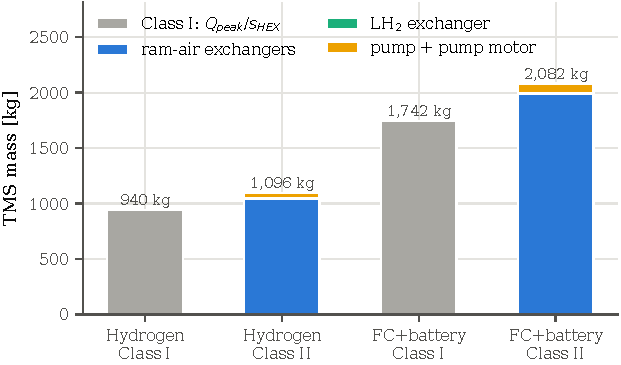
\includegraphics[width=0.72\textwidth]{mass_breakdown.pdf}
\caption{TMS mass on the reference designs. Class~I is $\max(\Qfc)/\SI{5}{kW/kg}$. The
Class-II mass is dominated by the ram-air exchangers; the LH$_2$ exchanger (\SI{3.8}{kg}
and \SI{7.2}{kg}) is too small to be visible.}
\label{fig:mass}
\end{figure}

Figure~\ref{fig:mass} shows the breakdown. The ram-air exchangers make up 95\,\% of the
Class-II mass on both aircraft. The pump and its motor are about 4\,\%, the LH$_2$
exchanger well below 1\,\%.

\subsection{Heat profile}
Figure~\ref{fig:heat-profile} shows the fuel-cell heat along the H2 Class-II mission. The
heat follows the propulsive power. It is highest in the first two climb segments, where the
climb gradient is largest, and in the diversion climb. In cruise it falls to
\SI{1505}{kW}, a third of the climb peak. The thermal profile has 13 points: the
take-off/OEI point and the peaks of the 12 flown segments. The mission peak, \SI{4878}{kW},
is reached at the start of \code{Mission/Climb2}, at \SI{1200}{m} and \SI{100}{m/s}, where
the speed steps up. The take-off/OEI point carries \SI{4177}{kW}, less than the climb peak.

\begin{figure}[htbp]
\centering
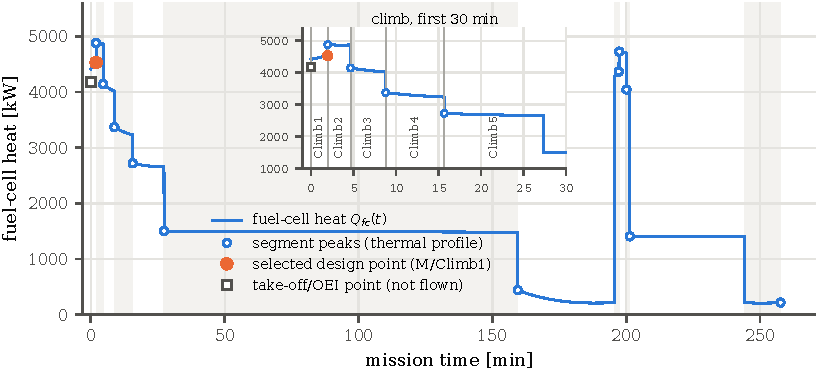
\includegraphics[width=\textwidth]{heat_profile.pdf}
\caption{Fuel-cell heat along the mission of the H2 Class-II design (the 420 accepted
solver points of the converged design, re-flown once), the 12 segment peaks of the thermal
profile and the take-off/OEI point placed at $t = 0$. Shaded bands mark alternate
segments. The inset enlarges the climb.}
\label{fig:heat-profile}
\end{figure}

\subsection{Design-point selection}
Nine of the 13 points carry at least half of the peak heat and become candidates.
Figure~\ref{fig:candidates} shows the mass of each candidate geometry and its worst
shortfall over the mission. Only the geometry sized at \code{Mission/Climb1}
(\SI{4531}{kW}, \SI{1208}{m}, \SI{80}{m/s}) rejects the heat at every point. It is not the
point with the most heat. It is the slowest high-heat point, so it has the least ram air
for a given capture area. Every other geometry falls short at \code{Mission/Climb1}: by
3.3\,\% for \code{Diversion/Climb1}, by 5.2\,\% for \code{Mission/Climb2} and by up to
50.3\,\% for \code{Mission/Climb5}. A heavier geometry is not automatically safe. The
take-off and \code{Mission/Climb2} geometries are the heaviest (\SI{1287}{kg} and
\SI{1286}{kg}) and still fall 12.3\,\% and 5.2\,\% short at \code{Mission/Climb1},
because their intakes were sized at the higher speeds of \SI{90}{m/s} and \SI{100}{m/s}.
The FCB Class-II design selects the same point with the same pattern. On all three
Class-II designs the rating along the continuous mission (step~5 of
Section~\ref{sec:design-point}) finds no shortfall above the tolerance, so it adds no
candidate.

\begin{figure}[htbp]
\centering
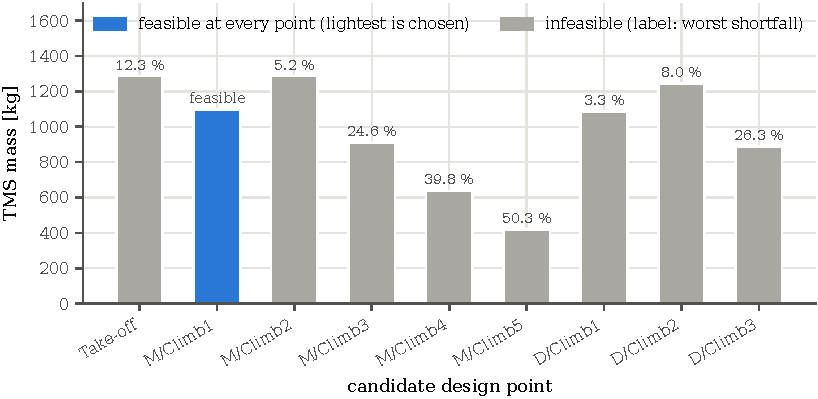
\includegraphics[width=\textwidth]{candidates.pdf}
\caption{Design-point selection of the H2 Class-II design: TMS mass of the geometry sized
at each candidate point, and its worst relative shortfall when rated at every mission
point. The worst shortfall of every infeasible candidate occurs at \texttt{Mission/Climb1}.}
\label{fig:candidates}
\end{figure}

\subsection{The sized hardware}
At the design point the stack heat is \SI{4531}{kW}. The reactants absorb \SI{85}{kW}
(1.9\,\%), HEX~1 transfers \SI{343}{kW} (7.6\,\%) to the hydrogen and HEX~2 rejects
\SI{4104}{kW} to ram air. The coolant flow is \SI{114.7}{kg/s}. The ram-air flow is
\SI{81.5}{kg/s} through a capture area of \SI{0.936}{m^2}.

\begin{itemize}
\item \textbf{HEX~1} is one plate-fin unit of \SI{3.81}{kg} and \SI{9.2}{L}: 36 layers,
  \SI{0.3}{m} wide, \SI{65}{mm} flow length, fin pitch \SI{1.5}{mm}, fin height
  \SI{6}{mm}. Its reference area is \SI{7.05}{m^2} and $U = \SI{388}{W/(m^2K)}$. Its
  coolant-side pressure drop is \SI{192}{Pa}, so HEX~2 may use the remaining
  \SI{199.8}{kPa} of the pump rise. The best finned and plain tube banks for the same duty
  weigh \SI{8.4}{kg} and \SI{20.6}{kg}.
\item \textbf{HEX~2} is 31 finned-tube-bank units of \SI{33.7}{kg} and \SI{49.9}{L} each,
  so the volume cap of \SI{50}{L} sets the unit count. Each unit has 261 tubes of
  \SI{6}{mm} outer diameter (29 per row, 9 rows, \SI{0.54}{m} long, 167 coolant circuits),
  with aluminium fins \SI{6}{mm} high at 650 fins/m. Its reference area is
  \SI{43.2}{m^2} with $U = \SI{90.6}{W/(m^2K)}$. The core air velocity is \SI{16.2}{m/s},
  the air-side pressure drop \SI{319}{Pa} and the coolant-side pressure drop \SI{9.9}{kPa}.
  The finned tube bank is the only family with a feasible design for this role.
\item \textbf{Pump}: \SI{32.0}{kW} electrical and \SI{46.5}{kg}.
\end{itemize}

\begin{figure}[htbp]
\centering
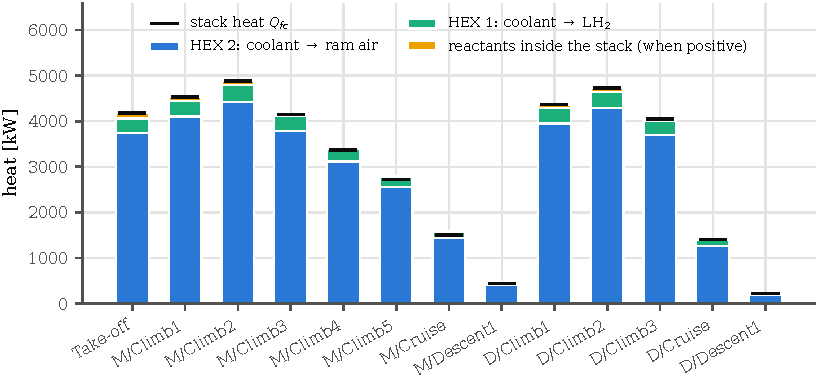
\includegraphics[width=\textwidth]{heat_split.pdf}
\caption{Heat split at every point of the H2 Class-II thermal profile
(\texttt{TMS.\_conditions}). Where the black mark lies below the top of the bar, the
reactant term~\eqref{eq:qreact} is negative: the compressed cathode air is hotter than
$T_{op}$ and the coolant must reject more than the stack heat.}
\label{fig:heat-split}
\end{figure}

Figure~\ref{fig:heat-split} shows the same split at every point. The hydrogen absorbs
between 7.4 and 11.6\,\% of the stack heat along the mission (the larger shares at the
low-power cruise and descent points), so the ram air rejects most of it. The reactant term
changes sign with altitude. Near the ground it removes up to \SI{117}{kW} at take-off. At
\code{Mission/Climb4} (\SI{4200}{m}) and above, the compressor delivery temperature exceeds
$T_{op}$, and the cathode air adds up to \SI{75}{kW} in cruise.

\begin{figure}[htbp]
\centering
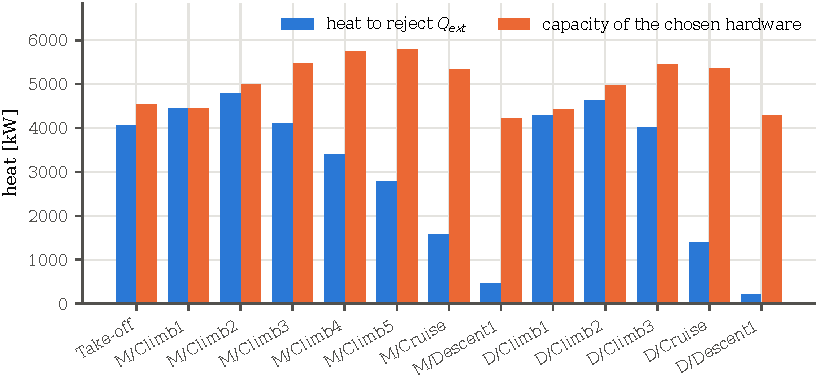
\includegraphics[width=\textwidth]{rating.pdf}
\caption{The chosen H2 Class-II hardware rated at every mission point: heat to reject and
full capacity (\texttt{RateAtPoint(..., capped=False)}).}
\label{fig:rating}
\end{figure}

Figure~\ref{fig:rating} rates the chosen hardware over the mission. The capacity equals
the requirement at the design point (\SI{4446}{kW}). The margin is small at
\code{Diversion/Climb1} (\SI{4431}{kW} against \SI{4283}{kW}) and 12\,\% at take-off
(\SI{4542}{kW} against \SI{4060}{kW}). At cruise the hardware could reject more than three
times the heat (\SI{5345}{kW} against \SI{1580}{kW}), because the air is colder and the
intake, whose area does not change, captures more air at the higher speed.

\subsection{Check along the mission}\label{sec:checkresults}
\code{CheckMission} checks the chosen hardware at the 13 profile points and at the 420
integration points of the H2 mission (423 on FCB). Table~\ref{tab:checks} summarizes it.
On all three designs the hardware rejects the heat everywhere: the worst shortfall along
the mission is 0.15\,\% (H2 with $\eta_{ram} = 0.9$). The coolant-side drop of the two
cores is about \SI{10}{kPa}, 5\,\% of the \SI{200}{kPa} budget. At 71 points of the H2
missions (72 on FCB), all in the descents, the low hydrogen flow takes the plate-fin
hydrogen side out of the Manglik and Bergles range, so the coolant drop there is unknown.
The air-side drop of the ram-air core reaches at most 10\,\% of the recovered dynamic
pressure, at \code{Mission/Climb1}. The duct does not choke at any point. The lowest
coolant-side wall temperature~\eqref{eq:twall} is \SI{274.9}{K} to \SI{275.0}{K}, at the
peak of \code{Mission/Climb2}, \SI{16}{K} above the freezing point of the coolant
(\SI{258.6}{K}).

With the ideal intake the duct drag is zero everywhere. With $\eta_{ram} = 0.9$ the
design-point drag is \SI{168}{N}. Over the mission the momentum balance gives a duct drag
work of \SI{15.1}{MJ}, while the constant $\Delta C_D$ charges \SI{376.9}{MJ}. In cruise and
descent the heat is low and the flap throttles the intake, so the duct drag falls much faster
than the dynamic pressure. The constant $\Delta C_D$ is therefore conservative over the
mission. Locally it can be slightly optimistic: at 39 of the 433 points, all near the start
of \code{Mission/Climb1}, the momentum balance gives more, by at most \SI{71}{N}
(\SI{259}{N} against \SI{187}{N}). The aircraft drag there is about \SI{11.7}{kN}
(level-flight lift coefficient), so the difference is \SI{0.6}{\%} of it, below the accuracy
of the drag polar.

\begin{table}[htbp]
\centering\small
\caption{Check of the chosen Class-II hardware at every profile and integration point
(\texttt{CheckMission}), default TMS inputs except $\eta_{ram}$.}\label{tab:checks}
\begin{tabular}{@{}lrrr@{}}
\toprule
 & H2 II & H2 II, $\eta_{ram}$\,0.9 & FCB II \\
\midrule
Checked points                        & 433 & 433 & 436 \\
Worst heat shortfall [\%]             & 0.02 & 0.15 & 0.02 \\
Max coolant drop of the cores [kPa]   & 10.1 & 10.0 & 10.0 \\
Max air drop / recovered $q_\infty$   & 0.091 & 0.101 & 0.091 \\
Choked points                         & 0 & 0 & 0 \\
Duct drag work, momentum [MJ]         & 0 & 15.1 & 0 \\
Duct drag work, $\Delta C_D$ [MJ]     & 0 & 376.9 & 0 \\
Lowest coolant-side wall [K]          & 274.9 & 275.0 & 275.0 \\
\bottomrule
\end{tabular}
\end{table}

\paragraph{Freezing at a lower intake recovery.} The regression design of
\code{test_tms_design.py::test_ram_drag_feeds_back_as_a_drag_increment}, the hydrogen test
aircraft of \code{tests/regression/test_hydrogen.py} with $\eta_{ram} = 0.8$ (rerun by
\code{compute_data.py:freezing_design}), flags the freezing risk: the estimated coolant-side wall reaches \SI{248.9}{K} at take-off,
\SI{9.7}{K} below the freezing point, at 80 points of take-off and climb. The margin is of
the order the estimate cannot resolve, so the flag means that HEX~1 of this design needs a
finer model or an architecture that keeps the coolant away from the cryogenic hydrogen (an
intermediate loop or a hydrogen preheater, neither of which is modelled).

\subsection{Ram-air flow and drag of the sized duct}\label{sec:ramresults}
Figure~\ref{fig:ram} takes the ram-air exchanger of the H2 Class-II design with
$\eta_{ram} = 0.9$ and moves it over altitude and speed. The intake flow is
$\rho_\infty V_\infty A_{cap}$ with the flap fully open. The core velocity and pressure drop
come from the built geometry (\code{compute_U}). The heat is the design ram-air duty, or the
capacity where that is lower. The drag comes from \code{ram_air_drag}.

\begin{figure}[htbp]
\centering
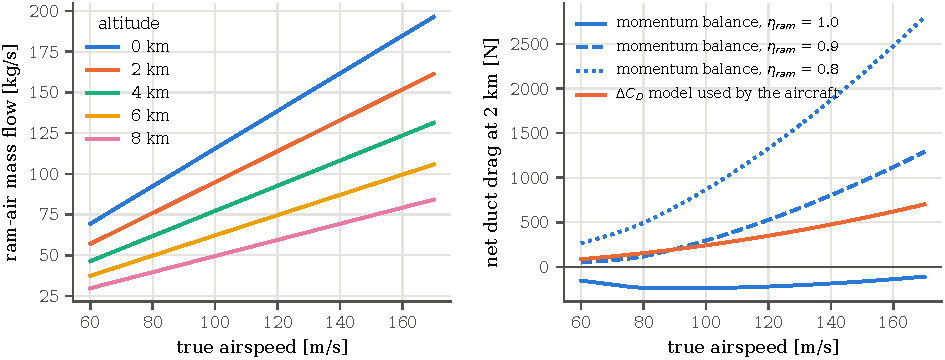
\includegraphics[width=\textwidth]{ram_sweep.pdf}
\caption{Frozen ram-air exchanger of the H2 Class-II design with $\eta_{ram} = 0.9$
(capture area \SI{0.943}{m^2}). Left: intake mass flow. Right: net duct drag at
\SI{2}{km} from the momentum balance~\eqref{eq:dram} for three intake recoveries, and the
drag that the aircraft model applies through $\Delta C_D$~\eqref{eq:dcd}.}
\label{fig:ram}
\end{figure}

The mass flow scales with $\rho_\infty V_\infty$, from \SI{57}{kg/s} at \SI{60}{m/s} to
\SI{157}{kg/s} at \SI{165}{m/s} at \SI{2}{km}. The drag depends strongly on the intake
recovery. With an ideal intake the duct gives a net thrust of 120 to \SI{240}{N} at
\SI{2}{km}. With $\eta_{ram} = 0.9$ the drag grows from \SI{49}{N} at \SI{60}{m/s} to
\SI{1205}{N} at \SI{165}{m/s}; with $\eta_{ram} = 0.8$, from \SI{266}{N} to \SI{2638}{N}.
The constant-$\Delta C_D$ model of the aircraft gives 87 to \SI{661}{N}. It is close to the
momentum balance near \SI{90}{m/s} and underestimates it at high speed by about a factor
of two. Two caveats apply. First, the sweep keeps the flap fully open, while a real duct
would throttle the flow at high speed. Second, in cruise the heat is a third of the design
heat, which the sweep does not reduce. The comparison therefore bounds the error of the
$\Delta C_D$ model; it is not a mission drag estimate.

\subsection{Sensitivity to the TMS inputs}\label{sec:sens}
Figure~\ref{fig:sens} repeats \code{SizeForMission} on the frozen thermal profile of the
converged H2 Class-II design, changing one input at a time. The aircraft is not re-closed,
so the pump power and drag feedbacks are not included.

\begin{figure}[htbp]
\centering
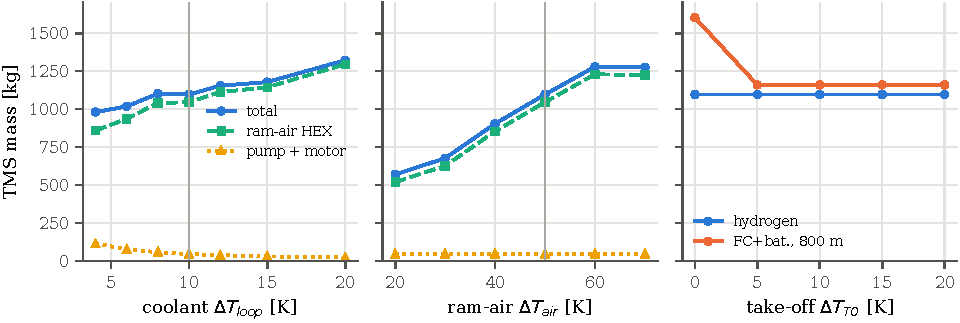
\includegraphics[width=\textwidth]{sensitivity.pdf}
\caption{TMS mass from \texttt{SizeForMission} on a frozen thermal profile. Left and
centre: H2 Class-II profile; the vertical line marks the default. Right: take-off coolant
over-temperature on the H2 Class-II profile and on the FCB-800 profile.}
\label{fig:sens}
\end{figure}

\paragraph{Coolant temperature drop.} From $\Delta T_{loop} = \SI{4}{K}$ to \SI{20}{K} the
TMS mass grows from \SI{981}{kg} to \SI{1322}{kg}. A smaller drop means a larger coolant
flow, a higher mean coolant temperature in HEX~2 and a larger driving temperature
difference, so the ram-air exchangers get lighter (\SI{859}{kg} at \SI{4}{K} against
\SI{1296}{kg} at \SI{20}{K}). The pump mass moves the other way (\SI{116}{kg} against
\SI{23}{kg}), and the pump power from \SI{80.1}{kW} to \SI{16.0}{kW}. The curve is not
monotone at \SI{8}{K} (\SI{1102}{kg} against \SI{1096}{kg} at \SI{10}{K}); this comes from
the discrete unit counts and candidate grids. Marconi~\cite{marconi2026} found an interior
optimum of the TMS mass in $\Delta T_{loop}$. The frozen-profile sweep shows no such
optimum between 4 and \SI{20}{K}. A closed design would add the cost of the pump power,
which grows five-fold from \SI{20}{K} to \SI{4}{K}, through the stack and the hydrogen.

\paragraph{Ram-air temperature rise.} A larger design rise needs less air but a higher
effectiveness. From \SI{20}{K} to \SI{60}{K} the ram-air flow falls from \SI{204}{kg/s} to
\SI{74}{kg/s} and the capture area from \SI{2.34}{m^2} to \SI{0.85}{m^2}, while the TMS
mass grows from \SI{571}{kg} to \SI{1280}{kg}. Beyond about \SI{55}{K} the cap
$\varepsilon_{max}(T_1 - T_{0,\infty})$ of~\eqref{eq:dtair} binds at the design point
($T_1 - T_{0,\infty} \approx \SI{69}{K}$, so the cap is \SI{55}{K}), so \SI{60}{K} and
\SI{70}{K} give the same air flow and almost the same mass. The input therefore trades
exchanger mass against intake size and drag. With the ideal intake the frozen-profile
sweep cannot price the drag.

\paragraph{Stack and piping pressure drop.} The H2 cores lose about \SI{10}{kPa} on the
coolant side, so a stack and piping share of up to \SI{180}{kPa} leaves the design
unchanged (\SI{1096}{kg}). With \SI{190}{kPa} the ram-air role needs 47 shorter units and
the TMS weighs \SI{1308}{kg}. With \SI{195}{kPa} it needs the maximum of 100 units, the
design point moves to \code{Diversion/Climb1} (\SI{1782}{kg}), and no candidate rejects
the heat at every point. The value of the input matters only when it leaves the cores less
than their pressure drop at the default budget.

\paragraph{Take-off coolant over-temperature.} On the H2 profile the over-temperature has
no effect, because \code{Mission/Climb1} sets the design. On the FCB-800 profile the
take-off point sets it: the larger take-off power of the \SI{800}{m} field gives a take-off
heat of \SI{5179}{kW} at \SI{90}{m/s}, close to the mission peak of \SI{5338}{kW}. With
$\Delta T_{TO} = 0$ the TMS is sized at take-off and weighs \SI{1602}{kg}. With
$\Delta T_{TO} = \SI{5}{K}$ the design moves to \code{Mission/Climb1} and the mass drops to
\SI{1160}{kg} ($-28$\,\%). Larger values change nothing more. This confirms the statement of
the user guide: the lever works only when the take-off point limits the design.

\subsection{Degraded fuel cell}\label{sec:degradation}
\code{FuelCell.set_state_of_health} (its docstring cites the voltage-decay approach of
Pessot et al.~\cite{pessot}) degrades the polarization curve of a sized stack. A uniform
cell-voltage loss increases the current for the same power, and by~\eqref{eq:qfc} each
ampere also carries more heat. Hence a degraded stack rejects much more heat at the same
propulsive power.

We flew the FCB-800 design (\code{examples/30_off_design_mission.py:fc_battery_design},
Class-I TMS) at its design take-off mass with a \SI{50}{mV} loss. The design heat, the
larger of the take-off and mission peak, is \SI{5338}{kW}. The degraded peak is
\SI{8366}{kW} (+57\,\%), and the degraded take-off heat \SI{7472}{kW} against
\SI{5179}{kW} (+44\,\%). \texttt{fly\_off\_design(sized, 750, state\_of\_health=\{"fc\_voltage\_loss": 0.05\})}
iterates the take-off mass and reports \SI{8649}{kW} against \SI{5338}{kW} (+62\,\%). It
also reports that the take-off mass, the fuel load and the battery power are exceeded, but
by at most 6.3\,\% (the fuel load, \SI{542}{kg} against \SI{510}{kg}). The heat limit is exceeded by far the most, so the TMS is the first system to
bind in a degraded flight.

\begin{figure}[htbp]
\centering
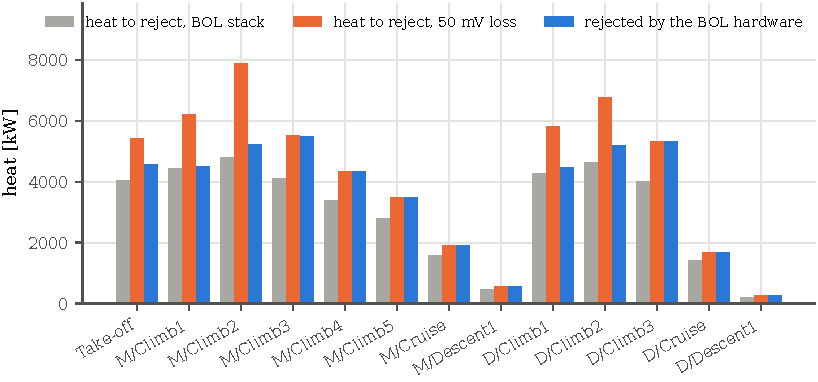
\includegraphics[width=\textwidth]{degradation.pdf}
\caption{H2 Class-II hardware (sized at beginning of life, BOL) with the stack degraded by
a \SI{50}{mV} cell-voltage loss, flown at the design take-off mass: heat to reject before
and after the degradation, and heat the BOL hardware rejects (\texttt{RateAtPoint}).}
\label{fig:degradation}
\end{figure}

For a Class-II design the hardware is rated directly. Figure~\ref{fig:degradation} flies
the H2 Class-II design at its design take-off mass with the same \SI{50}{mV} loss and rates
its BOL hardware. The heat to reject at \code{Mission/Climb2} grows from \SI{4788}{kW} to
\SI{7890}{kW} (+65\,\%). The hardware falls short by 33.9\,\% there, by 27.6\,\% at
\code{Mission/Climb1}, by 23.4\,\% at \code{Diversion/Climb2}, by 23.1\,\% at
\code{Diversion/Climb1} and by 15.5\,\% at take-off. From \code{Mission/Climb3} on, the
margin of the colder, faster points absorbs the extra heat (0.1\,\% short at
\code{Mission/Climb3}, none above it).

\code{fly_off_design} applies this rating itself when the design has a Class-II TMS
(\code{_tms_violation}): it runs \code{CheckAtPoint} with \code{weight.tms_result} at every
point of the flown thermal profile and every integration point of the flown mission, and
reports each broken limit of Section~\ref{sec:check} as a violation and each flagged risk in
\code{risks}. A Class-I design keeps the peak-heat comparison, since it has
no hardware to rate. The rating matters because the Class-II hardware has zero margin at
its design point and large margins elsewhere: the peak heat alone does not say where the
hardware falls short. On the H2 Class-II design, \code{fly_off_design} at \SI{750}{nmi}
reports no violation at beginning of life. With the \SI{50}{mV} loss it reports the
hardware short by 35\,\% at an integration point \SI{118}{s} into \code{Mission/Climb1},
together with a take-off mass and a fuel load (+6.3\,\%) above their design values and a
stack at 1.002 of its deliverable power. No other limit of Section~\ref{sec:check} is broken
and no risk is flagged. In the degraded flight at the design take-off mass, 91 of
the 441 checked points fall short of heat, and the lowest coolant-side wall is
\SI{266.5}{K}, still above the freezing point.

\subsection{Cost}
The Class-II designs took 112 to \SI{157}{s} and the Class-I designs 26 to \SI{30}{s}
(Table~\ref{tab:designs}). On the converged H2 Class-II design, one \code{SizeForMission}
takes \SI{1.16}{s} on the 13-point profile and \SI{1.25}{s} with the 420 integration
points added, so the continuous rating costs about \SI{0.09}{s} per call. The closure calls
\code{SizeForMission} once per fuel-cell pass, up to six passes per take-off-weight
evaluation. \code{CheckMission} on the 433 points takes \SI{0.33}{s} and runs once per
design. The hydrogen properties of HEX~1 depend only on $T_{op}$ and the inputs, so
\code{TMS._hydrogen_properties} evaluates them once per coolant temperature and keeps them.


%% ======================================================================================
\section{Usage}\label{sec:usage}
%% ======================================================================================

This section shows how to select the TMS class, read the results and use the Class-II model
on its own. The snippets run from \code{trunk/} with the package installed in the
\code{phlygreen} environment.

\subsection{Typed configuration}
A \code{TMSConfig} is attached to the \code{AircraftConfig} of a fuel-cell aircraft. Every
field except \code{tms_class} is optional; \code{None} keeps the model default. The
reference configurations of \code{examples/common.py} take a \code{tms_class} argument,
which attaches \code{common.tms_config(tms_class)}: a \code{TMSConfig} with every input
written out at its default value. It is a convenient starting point for changes.
\begin{lstlisting}
import sys; sys.path.insert(0, 'examples')
import PhlyGreen as pg
from PhlyGreen.config import TMSConfig
from common import hydrogen_config, fuelcell_battery_config, tms_config

config = hydrogen_config(tms_class='II')   # or fuelcell_battery_config(tms_class='II')
config.tms.ram_recovery = 0.9              # intake recovers 90 % of the dynamic pressure

# equivalent, without the helper:
# config = hydrogen_config(); config.tms = TMSConfig(tms_class='II', ram_recovery=0.9)

aircraft = pg.build_aircraft()
aircraft.configure(config)                 # about 2 min with Class II

r = aircraft.results()
print(r.tms_class, r.tms_mass, r.tms_pump_power, r.tms_ram_drag, r.tms_design_point)
aircraft.tms.report()                      # units, families, pump, ram air, drag
\end{lstlisting}
Without a \code{TMSConfig} (or with \code{tms_class='I'}) the Class-I model runs. Its only
input is \code{EnergyConfig.hex_specific_power_h2}.

\subsection{Legacy dictionaries}
The same inputs go into the \code{TMSInput} dictionary of \code{DesignAircraft}:
\begin{lstlisting}
aircraft.DesignAircraft(AerodynamicsInput, ConstraintsInput, MissionInput, EnergyInput,
                        MissionStages, DiversionStages,
                        TMSInput={'TMS Class': 'II', 'TMS Ram Recovery': 0.9})
\end{lstlisting}
\code{ReadInput} does not keep a \code{TMSInput} from a previous call. A call without it
selects Class~I.

\subsection{Inputs}
Table~\ref{tab:inputs} lists every input. The defaults are those of
\code{ThermalManagementSystem.__init__}; \code{common.tms_config} repeats them. \code{TMSConfig.__post_init__} checks that the
class is \code{'I'} or \code{'II'}, that the temperature differences, caps, pressures and
specific powers are positive, that the over-temperature and the stack and piping pressure drop
are not negative, that the latter is below the loop pressure rise when both are given, and
that the efficiencies, the ram recovery and the maximum effectiveness lie in $(0, 1]$.
\code{SetInput} checks $0 \le \Delta p_{stack} < \Delta p_{loop}$ on the values it reads.

\begin{table}[htbp]
\centering\scriptsize
\caption{TMS inputs: \texttt{TMSConfig} field, legacy key of \texttt{TMSInput} (or
\texttt{EnergyInput} for the last two rows), default, units and meaning. Only
\texttt{tms\_class} and the specific powers apply to Class~I.}\label{tab:inputs}
\setlength{\tabcolsep}{3pt}
\begin{tabularx}{\textwidth}{@{}>{\raggedright\arraybackslash}p{3.4cm}>{\raggedright\arraybackslash}p{3.9cm}lp{0.9cm}>{\raggedright\arraybackslash}X@{}}
\toprule
Field & Legacy key & Default & Units & Meaning \\
\midrule
\code{tms_class} & \texttt{TMS Class} & \code{'I'} & -- & model class, \code{'I'} or \code{'II'} \\
\code{coolant} & \texttt{TMS Coolant} & \texttt{INCOMP::MEG-30\%} & -- & CoolProp name of the coolant \\
\code{coolant_delta_t} & \texttt{TMS Coolant DeltaT} & 10 & K & coolant temperature drop over the loop, $\Delta T_{loop}$ \\
\code{max_volume_per_unit} & \texttt{TMS Max Volume Per Unit} & 0.05 & m$^3$ & volume cap of one exchanger unit \\
\code{max_weight_per_unit} & \texttt{TMS Max Weight Per Unit} & 50 & kg & mass cap of one exchanger unit \\
\code{max_hex_units} & \texttt{TMS Max HEX Units} & 100 & -- & maximum parallel units per role \\
\code{ram_air_delta_t} & \texttt{TMS Ram Air DeltaT} & 50 & K & design ram-air temperature rise, $\Delta T_{air,design}$ \\
\code{ram_air_max_effectiveness} & \texttt{TMS Ram Air Max Effectiveness} & 0.8 & -- & cap $\varepsilon_{max}$ of the rise, as a fraction of $T_1 - T_{0,\infty}$ \\
\code{h2_approach_delta_t} & \texttt{TMS H2 Approach DeltaT} & 30 & K & H$_2$ leaves HEX~1 at $T_{op}$ minus this, $\Delta T_{H_2}$ \\
\code{h2_supply_pressure} & \texttt{TMS H2 Supply Pressure} & $1.6\times10^5$ & Pa & LH$_2$ enters HEX~1 saturated at this pressure \\
\code{loop_pressure_drop} & \texttt{TMS Loop Pressure Drop} & $2\times10^5$ & Pa & pump pressure rise, $\Delta p_{loop}$ \\
\code{stack_pressure_drop} & \texttt{TMS Stack And Piping Pressure Drop} & 0 & Pa & part of $\Delta p_{loop}$ taken by the stack channels and the piping, $\Delta p_{stack}$; the cores share the rest \\
\code{pump_efficiency} & \texttt{TMS Pump Efficiency} & 0.75 & -- & $\eta_{pump}$ \\
\code{pump_motor_efficiency} & \texttt{TMS Pump Motor Efficiency} & 0.95 & -- & $\eta_{motor}$ \\
\code{pump_specific_power} & \texttt{TMS Pump Specific Power} & 800 & W/kg & electrical power per pump mass, $s_{pump}$ \\
\code{pump_motor_specific_power} & \texttt{TMS Pump Motor Specific Power} & 5000 & W/kg & electrical power per motor mass, $s_{motor}$ \\
\code{ram_recovery} & \texttt{TMS Ram Recovery} & 1.0 & -- & fraction $\eta_{ram}$ of the dynamic pressure the intake recovers \\
\code{takeoff_coolant_overtemperature} & \texttt{TMS Takeoff Coolant Overtemperature} & 0 & K & coolant above $T_{op}$ at the take-off point only, $\Delta T_{TO}$ \\
\midrule
\code{EnergyConfig.hex_specific_power_h2} & \texttt{HEX Specific Power H2} & 5000 & W/kg & Class-I specific power $s_{HEX}$ \\
\code{EnergyConfig.hex_specific_power_battery} & \texttt{HEX Specific Power Battery} & 1500 & W/kg & Class-II battery cooling (battery manual) \\
\bottomrule
\end{tabularx}
\end{table}

Three constants are not exposed as inputs: \code{CANDIDATE_HEAT_FRACTION} = 0.5,
\code{FEASIBILITY_TOLERANCE} = 0.02 and \code{MAX_ADDED_CANDIDATES} = 3 are class attributes
of \code{ThermalManagementSystem}. The family grids, wall and fin materials, and design
velocities are class attributes and module constants of \code{hex.py}.

\subsection{Reading the result}
Table~\ref{tab:outputs} lists where the design exposes the TMS. The Class-II result is a
\code{FCThermalManagementResult}.

\begin{table}[htbp]
\centering\small
\caption{TMS outputs after a design.}\label{tab:outputs}
\begin{tabularx}{\textwidth}{@{}p{4.6cm}X@{}}
\toprule
Where & What \\
\midrule
\code{aircraft.results()} & \code{tms_class}, \code{tms_mass} [kg] (= \code{weight.WHeat_Exchanger}), \code{hex_mass} [kg] (the same term, the heat-exchanger mass of the closure), \code{tms_pump_power} [W], \code{tms_ram_drag} [N], \code{tms_design_point}, \code{fuelcell_rating} [W]; \code{empty_weight} [kg] contains the TMS mass with the structure, powertrain, crew, battery and H$_2$ tank \\
\code{aircraft.weight.WHeat_Exchanger} & TMS mass in the weight balance [kg] \\
\code{aircraft.weight.tms_result} & \code{FCThermalManagementResult} (Class~II), fields below \\
\quad\code{design_point} & the mission point the hardware was sized at (dictionary) \\
\quad\code{units} & list of \code{ExchangerUnit}: \code{role}, \code{design} (\code{HEX_Design}: \code{family}, \code{geometry}, \code{A}, \code{U}, \code{q}, \code{weight}, \code{volume}, \code{dP_hot}, \code{dP_cold}, \code{v_cold}), \code{n_parallel}, \code{q}, \code{mass}, \code{volume}, \code{caps_exceeded}, \code{candidates} (best design of each family) \\
\quad\code{mdot_coolant}, \code{mdot_ram_air} & coolant flow (fixed by the pump) and ram-air flow at the design point [kg/s] \\
\quad\code{capture_area} & intake capture area [m$^2$] \\
\quad\code{pump_power}, \code{pump_mass} & electrical pump power [W]; pump + motor mass [kg] \\
\quad\code{hex_mass}, \code{hex_volume} & exchanger cores [kg], [m$^3$] \\
\quad\code{total_mass} & \texttt{hex\_mass + pump\_mass} [kg] \\
\quad\code{ram_drag}, \code{ram_drag_raw} & drag used by the aircraft ($\ge 0$) and the raw momentum balance [N] \\
\quad\code{heat_balance} & \code{stack}, \code{reactants}, \texttt{HEX H2}, \texttt{HEX ram air}, \code{unmet} [W] \\
\quad\code{heat_shortfall}, \code{caps_exceeded} & unmet heat at the design point [W]; cap flag \\
\quad\code{candidates} & design-point selection table \\
\quad\code{checks}, \code{violations()}, \code{risks()} & \code{CheckAtPoint} at every profile and integration point (Section~\ref{sec:check}); one message per broken limit or flagged risk \\
\quad\code{ram_drag_work}, \code{ram_drag_work_accounted} & duct drag work over the mission: momentum balance and constant $\Delta C_D$ [J] \\
\code{aircraft.mission.thermal_profile} & the heat-load points \\
\code{aircraft.mission.thermal_history} & the same quantities at every accepted integration point, with the time \code{t} \\
\code{aircraft.fuelcell.P_aux_tms} & pump power carried by the fuel cell [W] \\
\code{aircraft.aerodynamics.extra_Cd} & drag increment~\eqref{eq:dcd} \\
\bottomrule
\end{tabularx}
\end{table}

The chosen hardware can be rated over the mission, and each unit drawn to scale:
\begin{lstlisting}
tms, res = aircraft.tms, aircraft.weight.tms_result
for p in aircraft.mission.thermal_profile:
    q_cap, q_req = tms.RateAtPoint(res, p, capped=False)   # capacity vs heat to reject
    print(f"{p['name']:20s} {q_req/1e3:7.0f} kW  {q_cap/1e3:7.0f} kW")
for c in res.candidates:                                    # design-point selection table
    print(c['point'], round(c['mass']), c['worst_shortfall'], c['feasible'])
for c in res.checks[:len(aircraft.mission.thermal_profile)]:  # operating state, profile points
    print(c['name'], c['dP_air'], c['dP_air_available'], c['ram_drag'], c['T_wall_min'], c['limits'])
print(res.violations(), res.risks())                        # broken limits, flagged risks

from PhlyGreen.Systems.Thermal.plotting import draw_hex, plot_tms_rating
for u in res.units:
    draw_hex(u.design, n_parallel=u.n_parallel).savefig(f"{u.role}.pdf")
\end{lstlisting}

\subsection{Sizing at a single point}
The subsystem also works outside the weight loop, for trade studies at fixed heat loads.
After a Class-II design (so that \code{aircraft.tms} and \code{aircraft.fuelcell} hold their
inputs), any point dictionary can be sized and any result rated:
\begin{lstlisting}
point = {'name': 'climb', 'Q_fc': 4.0e6, 'altitude': 2000.0, 'V_inf': 100.0,
         'mdot_h2': 0.05}
res = tms.SizeAtPoint(point)                       # FCThermalManagementResult
print(res.total_mass, res.pump_power, res.ram_drag_raw)
q_rej, q_req = tms.RateAtPoint(res, {**point, 'altitude': 6000.0, 'V_inf': 130.0})

tms.coolant_delta_T = 15.0                         # change an input ...
res2 = tms.SizeForMission(aircraft.mission.thermal_profile)   # ... and re-select
\end{lstlisting}
\code{SizeForMission} on a frozen profile takes about one to two seconds. This is how the
sweeps of Section~\ref{sec:sens} were made. Such a sweep does not close the aircraft: the
heat profile, the stack and the take-off weight stay those of the original design. Reset the
modified attribute afterwards, because \code{SetInput} is the only place that restores it.

\subsection{Examples and tutorials}
\begin{itemize}
\item \code{examples/27_hydrogen_tms_class_ii.py} sizes the H2 aircraft with both classes,
  prints the design-point selection, rates the hardware over the mission, sweeps the ram
  recovery and draws both exchanger roles.
\item \code{tutorials/08_thermal_management.ipynb} walks through the heat source, the two
  classes, the heat split, the $\varepsilon$-NTU behaviour, the design-point choice and the
  trade between ram-air temperature rise and drag.
\item \code{examples/30_off_design_mission.py} flies frozen designs off-design. With a
  Class-II TMS it checks the design hardware (\code{CheckAtPoint}) over the flown thermal
  profile and every integration point of the flown mission; with Class~I it compares the
  peak heat with the design heat (Section~\ref{sec:degradation}).
\item \code{docs/user-guide/thermal-management.md} is the user guide.
\end{itemize}

\subsection{Pitfalls}
\begin{itemize}
\item \textbf{CoolProp.} Class~II needs CoolProp; \code{SetInput} raises an
  \code{ImportError} without it. The environment used here has CoolProp 7.2.0.
\item \textbf{Ideal intake.} With the default \texttt{ram\_recovery = 1} the momentum balance
  is usually a net thrust, so the drag passed to the aircraft is zero and the drag coupling
  is inactive. Use $\eta_{ram} < 1$ for a realistic duct.
\item \textbf{Cost.} A Class-II design takes about two minutes, against less than half a minute for
  Class~I (Section~\ref{sec:results}). Parameter sweeps over full designs should use
  Class~I or frozen-profile sweeps where possible.
\item \textbf{Warnings.} Check for the \code{RuntimeWarning}s of
  Section~\ref{sec:warnings}. A design with a shortfall or exceeded caps still closes.
\item \textbf{Coolant freezing.} HEX~1 faces hydrogen near \SI{20}{K} with a water--glycol
  coolant. The check of Section~\ref{sec:check} flags a risk when the estimated wall is below
  the freezing point; the sizing does not change the geometry to avoid it. With a coolant that
  has no CoolProp freezing data the check is skipped.
\item \textbf{Class-II battery.} In a fuel-cell + battery design with a Class-II battery,
  \code{tms_mass} and \code{hex_mass} also contain the battery cooling mass
  (Section~\ref{sec:battery-hex}).
\end{itemize}

%% ======================================================================================
\section{Verification and limitations}\label{sec:verification}
%% ======================================================================================

\subsection{Tests}
The following tests cover the TMS. We ran them on the code described here; all passed
(58 unit tests, the eight slow regression tests of \code{test_tms_design.py} and the 13
of \code{test_degradation.py}).
\begin{itemize}
\item \code{tests/unit/test_tms_components.py}: $\varepsilon$-NTU limits, textbook values
  and inversion; cross-flow labels; rating a sized unit at its design point returns the
  design duty for all three families; $U$ referred to the gas-side area; the selector
  picks the lightest family; per-unit caps; Meredith effect and drag trends of
  \code{ram_air_drag}; the hydrogen sink equals the CoolProp enthalpy rise with latent
  heat; the heat balance closes; mass is monotone in the heat load; the design-point
  selection is deterministic and feasible everywhere; $\Delta C_D$ uses the design-point
  dynamic pressure; the take-off over-temperature lightens a take-off design;
  \code{draw_hex} renders every family; an empty or heatless profile gives an empty TMS;
  thermal choking makes the ram-air core infeasible; the cores in series share the pump
  pressure rise; the stack and piping pressure drop shrinks the core budget only, and must
  leave a budget; \code{rate_unit} matches \code{rate_design} and gives the coolant-side
  film resistance; \code{CheckAtPoint} at the design point reproduces the sizing (heat,
  pressure drops, air flow, drag); it flags the air and coolant pressure budgets, the drag
  and the choking; the freezing point comes from CoolProp and the wall estimate lies between
  the stream temperatures; a continuous-mission point short of cooling becomes a candidate,
  and a history without shortfall leaves the selection unchanged; the flap throttles the
  intake to the required heat.
\item \code{tests/regression/test_tms_design.py} (slow): the factory wires the TMS; Class~I
  sizes on the larger of the mission and take-off heat; the Class-II hydrogen design
  closes; its geometry rejects the heat at every mission point; the ram drag feeds back as a
  drag increment; a $\phi = 0$ fuel-cell + battery design equals the hydrogen design, TMS
  included; the hardware is checked at every profile and integration point without a broken
  limit; the off-design check of example~30 reports the limits of \code{CheckAtPoint}.
\item \code{tests/regression/test_degradation.py} (slow): the Class-II hardware flown with a
  degraded stack is reported short of heat by \code{fly_off_design}, and the beginning-of-life
  flight is feasible.
\item \code{tests/unit/test_fuelcell_heat.py}: water saturation pressure, product-water
  vapour fraction and thermo-neutral voltages (heat source).
\item \code{tests/unit/test_thermal_network.py}: the \code{network.py} scaffold.
\end{itemize}
The numbers of Section~\ref{sec:results} add three consistency checks. First, the Class-I
masses equal the peak heat over \SI{5}{kW/kg} (\SI{4698.0}{kW} gives \SI{939.6}{kg} on H2,
\SI{8708.5}{kW} gives \SI{1741.7}{kg} on FCB). Second, the chosen hardware rejects exactly
the required heat at its design point (\SI{4446}{kW}), as the self-consistent sizing
requires. Third, \code{fly_off_design} flies the H2 Class-II design on its own mission
without any violation, including the limits of Section~\ref{sec:check}.

\subsection{Limitations}
\begin{itemize}
\item \textbf{Core-only mass.} Headers, manifolds, ducts, piping, coolant inventory and
  mounting structure are not included, and there is no fouling resistance.
\item \textbf{Stack and piping pressure drop.} The share of the loop pressure rise taken by
  the stack channels and the piping is an input with no sourced value; its default of zero
  gives the whole rise to the cores. The pump power uses the loop pressure rise, not the
  computed drops.
\item \textbf{Correlations.} The finned-bank air-side friction factor
  $f = 1.5\,Re^{-0.2}$ has no literature source (\code{hex.py} docstring). The candidate
  grids are coarse, so the mass moves in steps with the inputs
  (Section~\ref{sec:sens}).
\item \textbf{Hydrogen stream.} The hydrogen is a single stream with an effective specific
  heat and transport properties at its mean temperature. The boiling and the
  supercritical/gas regions are not resolved. Ortho--para conversion is not modelled.
\item \textbf{Drag.} The duct model has no spillage, cowl or wall losses beyond
  $\eta_{ram}$, and the default ideal intake usually gives zero drag. The drag enters the
  aircraft as a constant $\Delta C_D$, which follows the dynamic pressure but not the
  heat, the flap setting or the momentum balance (Section~\ref{sec:ramresults}). Over the
  mission it charges more drag work than the momentum balance; at single points it can charge
  slightly less. The constraint diagram does not see the duct drag.
\item \textbf{No fans and no transients.} Ground and low-speed points are cooled by ram air
  only; taxi is not in the thermal profile. The stack holds $T_{op}$ at all loads; thermal
  inertia and control are not modelled.
\item \textbf{Mission sampling.} The continuous check uses the accepted points of the
  mission integrator. Conditions between two accepted points are not rated.
\item \textbf{Coolant freezing.} The wall temperature~\eqref{eq:twall} pairs the coolant
  outlet with the cold-stream inlet; it does not resolve the temperature field of the core.
  A wall below the freezing point is reported as a risk, and the sizing does not change the
  geometry to avoid it. The freezing point is CoolProp's; fluids without CoolProp freezing data are
  not checked.
\item \textbf{Off-design limits are reported, not designed for.} The cores meet the
  pressure limits at their own design point, and the design-point selection rates the
  candidates on the heat only. Away from the design point, the pressure budgets, choking and
  freezing of Section~\ref{sec:check} are checked on the chosen hardware and reported; they
  do not change the selection.
\item \textbf{Defaults.} None of the TMS defaults is calibrated against flight hardware.
\end{itemize}

%\subsection{Differences from the thesis}\label{sec:thesis-diff}
%The code is the reference. Marconi's thesis~\cite{marconi2026} describes the method and an
%earlier state of the implementation. The main differences are:
%\begin{enumerate}
%\item \textbf{Design-point selection.} The thesis screens every phase with a quick
%  estimate, sizes the three best-scoring candidates in full and rates them against the
%  continuous, time-resolved mission. The code sizes every point carrying at least half of
%  the peak heat and rates each geometry at the discrete points of the thermal profile. It
%  rates the chosen geometry at every integration point of the mission and adds a point where
%  it falls short to the candidates.
%\item \textbf{Families.} The thesis considers four constructional families, adding the
%  plain plate exchanger to the three of the code. It selects the family on a
%  weight--volume Pareto front. The code keeps the lightest feasible family and uses the
%  Pareto front only for reporting.
%\item \textbf{Fallback.} When no geometry meets the caps, the thesis falls back to the
%  quick-screening estimate capped at the limits and tracks the unmet heat. The code sizes
%  the units without caps at \code{max_hex_units}, flags \code{caps_exceeded}, and records
%  a shortfall only when no family can do the duty at all.
%\item \textbf{Sub-iteration.} In the thesis the TMS is not sized on the first pass, the
%  drag increment is under-relaxed (equal blend with the previous value), and it is kept
%  across take-off-weight evaluations. The code sizes the TMS on every pass, sets the drag
%  increment without relaxation, and resets it at the start of each closure.
%\item \textbf{Class I.} The thesis writes the low-fidelity model as
%  $Q_{max}/(k_{TMS}\,\Delta T_{sizing})$; the code uses a specific power.
%\item \textbf{Materials.} The thesis states steel tubes and plates with aluminium fins. In
%  the code the plate-fin core is all aluminium.
%\end{enumerate}
%The thesis results (for example a \SI{2.6}{\%} MTOW increase over the linear model, with a
%diversion-climb design point) were obtained with other aircraft, stack and TMS inputs.
%They are not reproduced by the reference designs of this manual.


%% ======================================================================================
\begin{thebibliography}{99}\small
\bibitem{marconi2026} D.~Marconi. \emph{Geometrical Sizing of Thermal Management System for
  a Hydrogen Fuel Cell Regional Aircraft}. Master Thesis (Laurea Magistrale in Ingegneria
  Aeronautica), Dipartimento di Ingegneria Meccanica e Aerospaziale, Sapienza University of
  Rome. Advisor: Prof.~R.~Malpica Galassi. Academic Year 2025/2026. 
\bibitem{flyzero} Aerospace Technology Institute. \emph{FlyZero: Thermal management --
  roadmap report}. Technical Report FZO-PPN-COM-0019, ATI, London, 2022. 
\bibitem{incropera} F.~P.~Incropera (and D.~P.~DeWitt). \emph{Fundamentals of Heat and Mass
  Transfer}, 6th ed. Wiley, 2010. Table~11.3 for the $\varepsilon$-NTU relations and Table~7.6
  for the Zukauskas row correction.
\bibitem{kays} W.~M.~Kays and A.~L.~London. \emph{Compact Heat Exchangers}, 3rd ed. Krieger,
  1998. 
\bibitem{zukauskas} A.~\v{Z}ukauskas. Heat transfer from tubes in crossflow. In
  \emph{Advances in Heat Transfer}, vol.~8, pp.~93--160. Academic Press, 1972.
\bibitem{briggs} D.~E.~Briggs and E.~H.~Young. Convection heat transfer and pressure drop of
  air flowing across triangular pitch banks of finned tubes. \emph{Chemical Engineering
  Progress Symposium Series}, 59(41):1--10, 1963.
\bibitem{manglik} R.~M.~Manglik and A.~E.~Bergles. Heat transfer and pressure drop
  correlations for the rectangular offset strip fin compact heat exchanger.
  \emph{Experimental Thermal and Fluid Science}, 10(2):171--180, 1995.
\bibitem{gnielinski} V.~Gnielinski. New equations for heat and mass transfer in turbulent
  pipe and channel flow. \emph{International Chemical Engineering}, 16(2):359--368, 1976.
\bibitem{holman} J.~P.~Holman. \emph{Heat Transfer}. For the Jakob
  pressure-drop correlation of staggered tube banks.
\bibitem{pessot} Pessot et al. Development of an aging estimation tool for a PEM fuel cell
  submitted to a mission profile. \emph{Fuel Cells}, 2020. 
\end{thebibliography}

\end{document}
